\documentclass[9pt]{beamer}

%%%%%%%%%%%%%%%%%%%%%%%%%%%%%%%%%%%%%%%%%%%%%%%%%%%%%%%%%%%%%%%%%
%%%%%%%%%%%%%%%%%%%%%%%%%%%%%%%%%%%%%%%%%%%%%%%%%%%%%%%%%%%%%%%%%
%%%%%%%%%%%%%%%%%%%%%%%%%%%%%%%%%%%%%%%%%%%%%%%%%%%%%%%%%%%%%%%%%

\title{Higher-level rules for sequent calculus}
\author[Miller, Pimentel]{
	\emph{Dale Miller} \\ {\small \'Ecole Polytechnique, France} \\\ \\ 
	{\small Joint work with Elaine Pimentel}
}



%%%%%%%%%%%%%%%%%%%%%%%%%%%%%%%%%%%%%%%%%%%%%%%%%%%%%%%%%%%%%%%%%
%%% BEAMER SETTINGS
%%%%%%%%%%%%%%%%%%%%%%%%%%%%%%%%%%%%%%%%%%%%%%%%%%%%%%%%%%%%%%%%%


\usecolortheme{dolphin}
\useinnertheme{rounded}
\useoutertheme{infolines}

%\setbeamertemplate{blocks}[rounded]%[shadow]
\setbeamercolor{block body alerted}{bg=alerted text.fg!10}
\setbeamercolor{block title alerted}{bg=alerted text.fg!20}
\setbeamercolor{block body}{bg=structure!10}
\setbeamercolor{block title}{bg=structure!20}
\setbeamercolor{block body example}{bg=green!10}
\setbeamercolor{block title example}{bg=green!20}

\setbeamertemplate{headline}[default]
%\setbeamertemplate{footline}[frame number]
\setbeamertemplate{navigation symbols}{}

\setbeamertemplate{sections/subsections in toc}[sections numbered]
\setbeamertemplate{itemize item}[circle]
\setbeamertemplate{itemize subitem}[triangle]
\setbeamerfont{itemize item}{size=\large}
\setbeamerfont{itemize subitem}{size=\tiny}
\setbeamertemplate{enumerate item}[circle]

%\setbeamertemplate{navigation symbols}{}
%%\setbeamertemplate{blocks}[rounded][shadow=false]
%\setbeamertemplate{title page}[default][colsep=-4bp,rounded=true]
%%\setbeamertemplate{part page}[default][colsep=-4bp,rounded=true]
%\setbeamertemplate{section page}{
%	\begin{beamercolorbox}[center]{section title}%sep=8pt,wd=\textwidth,
%		\usebeamerfont{section title}\insertsection\par
%	\end{beamercolorbox}
%}
%
%\setbeamertemplate{footline}[frame number]
%
%\setbeamersize{text margin left=1cm}
%\setbeamersize{text margin right=1cm}
%
%\setbeamercolor{alerted text}{fg=blue}
%\setbeamercolor{title}{bg=Grey!10}
%\setbeamercolor{frametitle}{bg=Grey!10}
%%\setbeamercolor{sectiontitle}{fg=LightBlue,bg=Grey!10}
%%\setbeamercolor{headline}{bg=DarkBlue}

\definecolor{LightBlue}{rgb}{0,0,0.8}
\definecolor{DarkGreen}{rgb}{0.15,0.50,0.30}
\definecolor{DarkBlue}{rgb}{0.15,0.3,0.5}
\definecolor{Grey}{rgb}{0.50,0.50,0.50}

\definecolor{darkgreen}{rgb}{0,.3,0}
\definecolor{darkred}{rgb}{.5,0,0}
\definecolor{darkblue}{rgb}{0,0,.7}
\definecolor{darkvio}{rgb}{.5,0,.5}
\definecolor{darkorange}{rgb}{.8,0,.4}
\definecolor{lightgreen}{rgb}{0,.9,0}
\definecolor{itemblue}{rgb}{0,0,.4}
\definecolor{lightblue}{rgb}{0,0,.3}
\definecolor{bananamania}{rgb}{0.98, 0.91, 0.71}


\renewcommand{\emph}[1]{{\color{blue} #1}}
\newcommand{\empha}[1]{{\color{darkgreen} #1}}
\newcommand{\emphb}[1]{{\color{darkvio} #1}}
\newcommand{\emphdb}[1]{{\color{darkblue} #1}}
\newcommand{\emphdr}[1]{{\color{darkred} #1}}
\newcommand{\emphdo}[1]{{\color{darkorange} #1}}


\newcommand{\yellow}[1]{{\color{yellow} #1}}
\newcommand{\white}[1]{{\color{white} #1}}
\newcommand{\violet}[1]{{\color{violet} #1}}
\newcommand{\teal}[1]{{\color{teal} #1}}
\newcommand{\red}[1]{{\color{red} #1}}
\newcommand{\purple}[1]{{\color{purple} #1}}
\newcommand{\pink}[1]{{\color{pink} #1}}
\newcommand{\orange}[1]{{\color{orange} #1}}
\newcommand{\olive}[1]{{\color{olive} #1}}
\newcommand{\magenta}[1]{{\color{magenta} #1}}
\newcommand{\lime}[1]{{\color{lime} #1}}
\newcommand{\lightgray}[1]{{\color{lightgray} #1}}
\newcommand{\green}[1]{{\color{green} #1}}
\newcommand{\gray}[1]{{\color{gray} #1}}
\newcommand{\darkgray}[1]{{\color{darkgray} #1}}
\newcommand{\cyan}[1]{{\color{cyan} #1}}
\newcommand{\brown}[1]{{\color{brown} #1}}
\newcommand{\blue}[1]{{\color{blue} #1}}
\newcommand{\black}[1]{{\color{black} #1}}

\newcommand{\semitransp}[2][35]{\textcolor{fg!#1}{#2}}



%%%%%%%%%%%%%%%%%%%%%%%%%%%%%%%%%%%%%%%%%%%%%%%%%%%%%%%%%%%%%%%%%
%%% PACKAGES
%%%%%%%%%%%%%%%%%%%%%%%%%%%%%%%%%%%%%%%%%%%%%%%%%%%%%%%%%%%%%%%%%

\usepackage{proof}

%\usepackage{amssymb}
\usepackage{bm}
\usepackage{colonequals}

\usepackage[weather]{ifsym} %weather symbols
\usepackage{wasysym} %smiley

%\usepackage{array}
%\usepackage{multirow,bigdelim}

\usepackage{tikz}
\usetikzlibrary{arrows,shapes,backgrounds,positioning}%,shapes.callouts,shapes.geometric}
\tikzset{
	itria/.style={
		draw,dashed, %shape border uses incircle,
		isosceles triangle,shape border rotate=90,yshift=-7ex}
}


%\usepackage[curve]{xy}

%\usepackage{virginialake}
%\vlnostructuressyntax % to avoid conflicts with macros definition
%\vlnosmallleftlabels
%
\newcommand{\vlhtr}[2]{\vlpd{#1}{}{#2}}



%%%%%%%%%%%%%%%%%%%%%%%%%%%%%%%%%%%%%%%%%%%%%%%%%%%%%%%%%%%%%%%%%
%%% MACROS
%%%%%%%%%%%%%%%%%%%%%%%%%%%%%%%%%%%%%%%%%%%%%%%%%%%%%%%%%%%%%%%%%
\def\proofadjust{\vadjust{\nobreak\vskip-2.7ex\nobreak}}
\def\semiproofadjust{\vadjust{\nobreak\vskip-1.3ex\nobreak}}

\newcommand{\eg}{e.g.,}
\newcommand{\lP}{$\lambda$Prolog}

\newcommand{\axioms}{\mathcal{T}}
\newcommand{\tup}[1]{\langle #1\rangle}

\newcommand{\impl}{\supset}
\newcommand{\seq}{\vdash}

\newcommand{\limpl}{L{\impl}}

\newcommand{\relfo}{R}

\newcommand{\truen}{t^-}
\newcommand{\truep}{t^+}
\newcommand{\falsen}{f^-}
\newcommand{\falsep}{f^+}
\newcommand{\wedgep}{\wedge^{\!+}}
\newcommand{\wedgen}{\wedge^{\!-}}
\newcommand{\veep}{\vee^{\!+}}
\newcommand{\veen}{\vee^{\!-}}

\newcommand{\wedgepn}{\wedge^{\!\pm}}
\newcommand{\veepn}{\vee^{\!\pm}}

\newcommand{\Seq}[2]{#1\vdash #2}
\newcommand{\labelleft}[1]{\deduce[\hbox{#1}]{\strut}{}}

\newcommand{\jLf}[3]{#1\; {\Downarrow #2} \vdash #3}% left focused sequent
\newcommand{\jRf}[3]{#1 \vdash {#2 \Downarrow}\;#3}% right focused sequent
\newcommand{\jUnf}[4]{#1 \mathbin\Uparrow #2 \vdash  #3 \mathbin\Uparrow #4}% unfocused sequent

\newcommand{\jUnfG   }[2]{\jUnf{\Gamma}{#1}{#2}{{}}}           % unf sequ with \Gamma
\newcommand{\jUnfGamb}[1]{\Gamma\mathbin\Uparrow#1\vdash \Rscr}% unf sequ with \Gamma
\newcommand{\Rscr}{\Delta_1\mathbin\Uparrow\Delta_2}                % Used for an ambiguous rhs
\newcommand{\jLfG    }[1]{\jLf{\Gamma}{#1}{E}}                 % left foc seq with \Gamma 
\newcommand{\jRfG    }[1]{\jRf{\Gamma}{#1}}                    % right foc seq with \Gamma
\newcommand{\jUnfamb }[3]{#1\mathbin\Uparrow#2\vdash#3 \Rscr}  % unfocused sequent

\newcommand{\krelease}{\mathsf{R}}
\newcommand{\kstore}{\mathsf{s}}
\newcommand{\kinit}{\mathsf{I}}

\newcommand\negclass[2]{\mathcal{N}_{#1}^{#2}}
\newcommand\posclass[2]{\mathcal{P}_{#1}^{#2}}

\newcommand{\xitem}{\pause\item}
\newcommand{\Ascr}{\mathcal{A}}
\newcommand{\Bscr}{\mathcal{B}}
\newcommand{\Cscr}{\mathcal{C}}

\newcommand{\fib}{\mathsf{fib}}


%%%%%%%%%%%%%%%%%%%%%%%%%%%%%%%%%%%%%%%%%%%%%%%%%%%%%%%%%%%%%%
%%%%%%%%%%%%%%%%%%%%%%%%%%%%%%%%%%%%%%%%%%%%%%%%%%%%%%%%%%%%%%
%%% General stuff
\newcommand*\mdelim[3]{%
	\mathopen{}\left#1%
	#3%
	\right#2\mathclose{}%
}

\newcommand*{\set}[1]{\mdelim{\lbrace}{\rbrace}{#1}}

\newcommand*{\EMP}{\varnothing}

%%%%%%%%%%%%%%%%%%%%%%%%%%%%%%%%%%%%%%%%%%%%%%%%%%%%%%%%%%%%%%
% focus
\newcommand*{\foc}[1]{{\fboxsep 1pt\fboxrule 0pt\fcolorbox{white}{blue!08}{$\langle#1\rangle$}}}
\def\posf#1{\textcolor{DarkGreen}{#1}}
\def\negf#1{\textcolor{orange}{#1}}
%%%%%%%%%%%%%%%%%%%%%%%%%%%%%%%%%%%%%%%%%%%%%%%%%%%%%%%%%%%%%%
%% First order
\newcommand*{\subst}[2]{(#1/#2)}
\newcommand*{\term}[1]{#1}%{\mathtt{#1}}%#1}%{

%%%%%%%%%%%%%%%%%%%%%%%%%%%%%%%%%%%%%%%%%%%%%%%%%%%%%%%%%%%%%%
%%%%%%%%%%%%%%%%%%%%%%%%%%%%%%%%%%%%%%%%%%%%%%%%%%%%%%%%%%%%%%
%%% Logic
\newcommand*{\ax}[1]{\mathsf{#1}}

\newcommand{\forcesym}{\Vdash}
%\newcommand{\nforcesym}{\nVdash}

\newcommand{\force}[2]{#1\forcesym#2}
%\newcommand{\nforce}[2]{#1\nforcesym#2}

%%%%%%%%%%%%%%%%%%%%%%%%%%%%%%%%%%%%%%%%%%%%%%%%%%%%%%%%%%%%%%
%%%%%%%%%%%%%%%%%%%%%%%%%%%%%%%%%%%%%%%%%%%%%%%%%%%%%%%%%%%%%%
%%% Systems
\newcommand*{\sys}[1]{\ensuremath{\mathsf{#1}}}%\xspace}


\newcommand*{\K}{\sys{K}}
%\newcommand*{\CK}{\sys{CK}}
\newcommand*{\IK}{\sys{IK}}
%\newcommand*{\X}{\sys{X}}

%\renewcommand*{\o}{\mathsf{o}}%{}%
%\newcommand*{\oK}{\o\K}
%\newcommand*{\oKf}{\o\sys{K4}}
%\newcommand*{\oKff}{\o\sys{K45}}
%\newcommand*{\oIK}{\o\IK}

%\newcommand*{\h}{\mathsf{h}}%{}%
%\newcommand*{\hK}{\h\K}
%\newcommand*{\hSfour}{\h\sys{S4}}

%\newcommand*{\lab}{\mathsf{lab}}
%\newcommand*{\labK}{\lab\K}
%\newcommand*{\labIK}{\lab\IK}

\newcommand*{\n}{\mathsf{n}}%{}%
\newcommand*{\nK}{\sys{n}\K}
%\newcommand*{\nK'}{\sys{n}\K'}
%\newcommand*{\nIK}{\sys{n}\IK}

\newcommand*{\f}{\mathsf{f}}
\newcommand*{\fnK}{\f\nK}
%\newcommand*{\fnIK}{\f\nIK}

\newcommand*{\wf}{\mathsf{w}}
\newcommand*{\wfnK}{\wf\nK}

\newcommand*{\s}{\mathsf{s}}
\newcommand*{\snK}{\s\nK}
%\newcommand*{\snIK}{\s\nIK}

%\newcommand*{\ii}{\mathsf{i}}
%\newcommand*{\inK}{\ii\nK}
%\newcommand*{\inIK}{\ii\nIK}
%\newcommand{\iinK}{\iddot\nK}
%\newcommand{\iinIK}{\iddot\nIK}

\newcommand*{\LK}{\sys{LK}}
\newcommand*{\LJ}{\sys{LJ}}
\newcommand*{\LKF}{\sys{LKF}}
\newcommand*{\LJF}{\sys{LJF}}
%\newcommand*{\LMF}{\sys{LMF}}
%\newcommand*{\LMFstar}[1][]{\LMF_\ast^{\mathsf{#1}}}
%\newcommand*{\LMFo}[1][]{\LMF_\o^{\mathsf{#1}}}
%%\newcommand*{\aLKF}{\hbox{\sys{LKF}\kern-2pt$^a$}}

%%%%%%%%%%%%%%%%%%%%%%%%%%%%%%%%%%%%%%%%%%%%%%%%%%%%%%%%%%%%%%
%%%%%%%%%%%%%%%%%%%%%%%%%%%%%%%%%%%%%%%%%%%%%%%%%%%%%%%%%%%%%%
%%% Connectives

\newcommand*{\NEG}[1]{\bar{#1}}
%\newcommand*{\NOT}{\neg}

\newcommand*{\AND}{\mathbin{\scalebox{.85}{$\wedge$}}}%{\mathbin{\scalebox{.85}{\raise.1ex\hbox{\large$\wedge$}}}}
\newcommand*{\PAND}{%
	\mathbin{\smash{\scalebox{.65}{$\stackrel{\hbox{\scalebox{1}{\tiny$\bm+$}}}{\hbox{\large$\wedge$}}$}}}%
}
\newcommand*{\NAND}[1][]{%
	\mathbin{\smash{\scalebox{.65}{$\stackrel{\hbox{\scalebox{1}{\tiny$\bm-$}}}{\hbox{\large$\wedge$}}$}}_{#1}}%
}

\newcommand*{\TOP}{\mathord{\scalebox{.85}{$\top$}}}
\newcommand*{\PTOP}{%
	\mathord{\smash{\scalebox{.7}{$\stackrel{\hbox{\scalebox{1}{\tiny$\bm+$}}}{\hbox{\large$\top$}}$}}}%
}
\newcommand*{\NTOP}{%
	\mathord{\smash{\scalebox{.7}{$\stackrel{\hbox{\scalebox{1}{\tiny$\bm-$}}}{\hbox{\large$\top$}}$}}}%
}

\newcommand*{\OR}{\mathbin{\scalebox{.85}{$\vee$}}}%{\mathbin{\scalebox{.85}{\raise.1ex\hbox{\large$\vee$}}}}
\newcommand*{\POR}{%
	\mathbin{\smash{\scalebox{.7}{$\stackrel{\hbox{\scalebox{1}{\tiny$\bm+$}}}{\hbox{\large$\vee$}}$}}}%
}
\newcommand*{\NOR}{%
	\mathbin{\smash{\scalebox{.7}{$\stackrel{\hbox{\scalebox{1}{\tiny$\bm-$}}}{\hbox{\large$\vee$}}$}}}%
}

\newcommand*{\BOT}{\mathord{\scalebox{.85}{$\bot$}}}
%\newcommand*{\PBOT}{%
%	\mathord{\smash{\scalebox{.7}{$\stackrel{\hbox{\scalebox{1}{\tiny$\bm+$}}}{\hbox{\scalebox{1}{\large$\bm\bot$}}}$}}}%
%}
%\newcommand*{\NBOT}{%
%	\mathord{\smash{\scalebox{.7}{$\stackrel{\hbox{\scalebox{1}{\tiny$\bm-$}}}{\hbox{\large$\bm\bot$}}$}}}%
%}

\newcommand*{\IMP}{\mathbin{\scalebox{.85}{\raise.2ex\hbox{$\supset$}}}}%{\mathbin{\scalebox{.6}{\raise.4ex\hbox{\large$\bm\supset$}}}}%\supset}}%

\newcommand*{\BOX}{\Box}%{\mathord{\medsquare}}
\newcommand*{\DIA}{\Diamond}%{\mathord{\scalebox{.9}{\raise.2ex\hbox{$\meddiamond$}}}}

\newcommand*{\SHP}{\mathord{\scalebox{.8}{\raise.2ex\hbox{\large$\downarrow$}}}}
\newcommand*{\SHN}{\mathord{\scalebox{.8}{\raise.2ex\hbox{\large$\uparrow$}}}}

\newcommand*{\FA}{\mathord{\scalebox{.9}{$\forall$}}}%{\mathord{\scalebox{.9}{\hbox{\large$\bm\forall$}}}}
\newcommand*{\EX}{\mathord{\scalebox{.9}{$\exists$}}}%{\mathord{\scalebox{.9}{\hbox{\large$\bm\exists$}}}}
%%%%%%%%%%%%%%%%%%%%%%%%%%%%%%%%%%%%%%%%%%%%%%%%%%%%%%%%%%%%%%
%%%%%%%%%%%%%%%%%%%%%%%%%%%%%%%%%%%%%%%%%%%%%%%%%%%%%%%%%%%%%%
%%% Rules
\newcommand*{\rn}[1]  {\ensuremath{\mathsf{#1}}}
%\newcommand*{\invr}[1]{{#1}^{-1}}

%\newcommand*{\rr}{\rn{r}}
\newcommand*{\id}{\rn{ax}}
%\newcommand*{\weak}{\rn{w}}
%\newcommand*{\cont}{\rn{c}}
%\newcommand*{\eweak}{\rn{ew}}
%\newcommand*{\econt}{\rn{ec}}
\newcommand*{\cut}{\rn{cut}}
\newcommand{\init}{\mathsf{init}}
%\newcommand*{\nec}{\rn{nec}}

%\newcommand\bcutr {\mathsf{cut_1}}
%\newcommand\fcutr {\mathsf{cut_2}}

%\newcommand*{\isub}{\rn{isub}}
%\newcommand*{\iid}{\rn{\iddot d}}
%\newcommand{\idia}{\hbox{$\ddot{\rlap{$\phantom{X}$}\DIA}$}}
%\newcommand{\ibox}{\hbox{$\ddot{\rlap{$\phantom{X}$}\BOX}$}}

%\newcommand\Xdia        {\nrn[X]\DIA}
%\newcommand\Xbr        {\nbrn{X}}

%\newcommand*{\grs}{\rn{grs}}
%\newcommand*{\urs}[1][]{\rn{urs_{#1}}}
%%%%%%%%%%%%%%%%%%%%%%%%%%%%%%%%%%%%%%%%%%%%%%%%%%%%%%%%%%%%%%
% Rules per systems
%\newcommand*{\orn}[2][]  {\rn{#2_{#1}^{\o}}} % ordinary seq
%\newcommand*{\hrn}[2][]  {\rn{#2_{#1}^{\h}}} % hyper seq
%\newcommand*{\labrn}[2][]  {\rn{#2_{#1}^{\lab}}} % labelled seq
%\newcommand*{\frn}[2][]  {\rn{#2_{#1}^{\f}}} % focused
\newcommand*{\nrn}[2][]  {\rn{#2_{#1}^{\n}}} % nested
\newcommand*{\fnrn}[2][]  {\rn{#2_{#1}^{\f\n}}} % focused nested
\newcommand*{\wfnrn}[2][]  {\rn{#2_{#1}^{\wf\n}}} % weakly focused nested
\newcommand*{\snrn}[2][]  {\rn{#2_{#1}^{\s\n}}} % synthetic nested
%\newcommand*{\inrn}[2][]  {\rn{#2_{#1}^{\ii\n}}} % indexed nested
%\newcommand*{\starn}[1]  {\mathsf{#1}_\ast} % LMF*
%%%%%%%%%%%%%%%%%%%%%%%%%%%%%%%%%%%%%%%%%%%%%%%%%%%%%%%%%%%%%%
% Structural rules
%\newcommand*{\brn}[2][]{\rn{#2_{#1}^{\hbox{$\scriptscriptstyle[\mkern2mu]$}}}}%
%\newcommand*{\brsym}{\mathord{\scalebox{.9}{$\BOXtimes$}}}
%\newcommand*{\brn}[1]{\rn{\brsym_{#1}}} % \blacksquare
%\newcommand*{\hbrn}[1]{\rn{\brsym_{#1}^{\h}}}
%\newcommand*{\nbrn}[1]{\rn{\brsym_{#1}^{\n}}}
%\newcommand*{\inbrn}[1]{\rn{\brsym_{#1}^{\ii\n}}}
%\newcommand*{\labbrn}[1]{\rn{\brsym_{#1}^{\lab}}}
%%%%%%%%%%%%%%%%%%%%%%%%%%%%%%%%%%%%%%%%%%%%%%%%%%%%%%%%%%%%%%
% Intuitionistic rules
\newcommand*{\rrn}[2][]  {\rn{#2_{R#1}}}
\newcommand*{\lrn}[2][]  {\rn{#2_{L#1}}}

%\newcommand*{\rlabrn}[2][]  {\rn{#2_{R#1}^\lab}}
%\newcommand*{\llabrn}[2][]  {\rn{#2_{L#1}^\lab}}

\newcommand*{\rnrn}[2][]  {\rn{#2_{R#1}^{\n}}}
\newcommand*{\lnrn}[2][]  {\rn{#2_{L#1}^{\n}}}

\newcommand*{\rfnrn}[2][]  {\rn{#2_{R#1}^{\f\n}}}
\newcommand*{\lfnrn}[2][]  {\rn{#2_{L#1}^{\f\n}}}

\newcommand*{\rsnrn}[2][]  {\rn{#2_{R#1}^{\s\n}}}
\newcommand*{\lsnrn}[2][]  {\rn{#2_{L#1}^{\s\n}}}

%\newcommand*{\rinrn}[2][]  {\rn{#2_{R#1}^{\ii\n}}}
%\newcommand*{\linrn}[2][]  {\rn{#2_{L#1}^{\ii\n}}}
%%%%%%%%%%%%%%%%%%%%%%%%%%%%%%%%%%%%%%%%%%%%%%%%%%%%%%%%%%%%%%
%%%%%%%%%%%%%%%%%%%%%%%%%%%%%%%%%%%%%%%%%%%%%%%%%%%%%%%%%%%%%%
%%% Nested sequents
\makeatletter
%\newcommand*\BR[2][]{\mdelim{\lbrack\strut^{#1}}{\rbrack}{#2}}
\newcommand*{\BR}{%
	\@ifnextchar\i{\br@two}{%
		\@ifnextchar\bgroup{\br@one}{% 
}}}
\newcommand*{\br@one}[1]{%
	\def\br@{#1}%
	\mdelim{\lbrack}{\rbrack}{\ifx\br@\empty\mkern 3mu\else #1\fi}%
}
\newcommand*{\br@two}[3]{%
	\def\br@{#3}%
	\mdelim{\lbrack\strut^{#2}}{\rbrack}{\ifx\br@\empty\mkern 3mu\else #3\fi}%
}

%\newcommand*{\@makeoperator}[2]{
%	\newcommand*{#1}{%
%		\mathrm{#2}\mdelim{\lparen}{\rparen}
%	}
%}
%\@makeoperator{\fm}{fm}
%\@makeoperator{\depth}{dp}
%\@makeoperator{\rank}{rk}
%\@makeoperator{\height}{ht}
%\@makeoperator{\tree}{tree}
%\@makeoperator{\graph}{graph}
\makeatother
%%%%%%%%%%%%%%%%%%%%%%%%%%%%%%%%%%%%%%%%%%%%%%%%%%%%%%%%%%%%%%
%contexts
\makeatletter
\newcommand*{\cxs}{%
	\@ifnextchar\i{\cxs@two}{%
		\@ifnextchar\bgroup{\cxs@one}{% % \bgroup is the same as {
}}}
\newcommand*{\cxs@one}[1]{%
	\def\cxs@{#1}%
	\mdelim{\lbrace}{\rbrace}{\ifx\cxs@\empty\mkern 3mu\else #1\fi}%
	\cxs@one@decor%
}
\newcommand*{\cxs@two}[3]{%
	\def\cxs@{#3}%
	\mdelim{\lbrace\strut^{#2}}{\rbrace}{\ifx\cxs@\empty\mkern 3mu\else #3\fi}%
	\cxs@one@decor%
}
\def\cxs@one@decor{%
	\@ifnextchar_{\cxs@one@sub}{%
		\@ifnextchar^{\cxs@one@sup}{%
			\@ifnextchar\dots{\@firstoftwo{\dotsm\cxs@one@decor}}{%
				\@ifnextchar[{\cxs@one@arg}%]
				\cxs}}}%
}
\def\cxs@one@sub_#1{_{#1}\cxs@one@decor}
\def\cxs@one@sup^#1{^{#1}\cxs@one@decor}
\def\cxs@one@arg[#1]{{#1}\cxs@one@decor}

%% Change these as needed, but keep the \cx@continuation at the end
\def\cx@delete@always#1{{#1}^{\ast}\cx@continuation}
\def\cx@delete@right#1*{{#1}^{\star}\cx@continuation}
\def\cx@delete@focus#1\f{{#1}^{\scriptscriptstyle\not{\langle}{\rangle}}\cx@continuation}

\def\cx@delete@star#1*{%
	\@ifnextchar*{\cx@delete@right{#1}}{\cx@delete@always{#1}}%
}

\newcommand*{\@makecontextual}[2]{
	\newcommand*{#1}{%
		\@ifnextchar*{\cx@delete@star{#2}}{%
			\@ifnextchar\f{\cx@delete@focus{#2}}{%
				#2\cx@continuation}}%
	}%
}
\newcommand*{\cx@continuation}[1][]{_{#1}\cxs}

\@makecontextual{\Ex}{}

\@makecontextual{\Cx}{\Gamma}%{{\color{DarkBlue}\Gamma}}
\@makecontextual{\Dx}{\Delta}%{{\color{DarkBlue}\Delta}}
\@makecontextual{\Lx}{\Lambda}%{{\color{DarkBlue}\Lambda}}
\@makecontextual{\Rx}{\Pi}%{{\color{DarkBlue}\Pi}}

\@makecontextual{\LLx}{\Omega}
\@makecontextual{\RRx}{\Xi}
\@makecontextual{\CCx}{\Sigma}
\@makecontextual{\DDx}{\Theta}
\makeatother
%%%%%%%%%%%%%%%%%%%%%%%%%%%%%%%%%%%%%%%%%%%%%%%%%%%%%%%%%%%%%%
%%%%%%%%%%%%%%%%%%%%%%%%%%%%%%%%%%%%%%%%%%%%%%%%%%%%%%%%%%%%%%
%%%%%%%%%%%%%%%%%%%%%%%%%%%%%%%%%%%%%%%%%%%%%%%%%%%%%%%%%%%%%%
%%% Synthetic
\newcommand*{\subf}{\mathbin{\setbox0=\hbox{$\in$}\copy0\kern-.8\wd0\box0}}
%\newcommand*{\srn}[1][]{\rn{\hbox{\tiny${\bm\langle}\mkern 1mu{\bm\rangle}$}_{#1}^{\s\n}}}
\newcommand*{\srn}[1][]{\rn{\DIAplus_{#1}^{\s\n}}}
\newcommand*{\syngen}[2] {\left\{ #1 \right\}_{#2}}
%%%%%%%%%%%%%%%%%%%%%%%%%%%%%%%%%%%%%%%%%%%%%%%%%%%%%%%%%%%%%%
% focus
\newcommand*{\sfoc}[1]{{\fboxsep 1pt\fboxrule 0pt\fcolorbox{white}{red!08}{$\langle#1\rangle$}}}
%%%%%%%%%%%%%%%%%%%%%%%%%%%%%%%%%%%%%%%%%%%%%%%%%%%%%%%%%%%%%%
%%%%%%%%%%%%%%%%%%%%%%%%%%%%%%%%%%%%%%%%%%%%%%%%%%%%%%%%%%%%%%
%%% Labels
\newcommand*{\Labx}{\mathcal{L}}
\newcommand*{\Rabx}{\mathcal{R}}
\newcommand*{\Gx}{\mathcal{G}}
\newcommand*{\labels}[2]{{\color{blue}{#1}\:\colon}{#2}}
\newcommand*{\rel}{R}
\newcommand*{\relp}{r}
\newcommand*{\CC}{\mathcal{C}}
%%%%%%%%%%%%%%%%%%%%%%%%%%%%%%%%%%%%%%%%%%%%%%%%%%%%%%%%%%%%%%
%%%%%%%%%%%%%%%%%%%%%%%%%%%%%%%%%%%%%%%%%%%%%%%%%%%%%%%%%%%%%%
%%% Translation 
%IK to LJF
\newcommand*{\trL}[2][]{\lfloor#2\rfloor_{#1}}
\newcommand*{\trR}[2][]{\lceil#2\rceil_{#1}}


%%%%%%%%%%%%%%%%%%%%%%%%%%%%%%%%%%%%%%%%%%%%%%%%%%%%%%%%%%%%%%%%%
%%%%%%%%%%%%%%%%%%%%%%%%%%%%%%%%%%%%%%%%%%%%%%%%%%%%%%%%%%%%%%%%%
%%%%%%%%%%%%%%%%%%%%%%%%%%%%%%%%%%%%%%%%%%%%%%%%%%%%%%%%%%%%%%%%%
%\usepackage{listings} % for listing code
%\input{listing-macros}
\newcommand{\adj}[2]{\hbox{\sl adj}~#1~#2}
\newcommand{\pth}[2]{\hbox{\sl path}~#1~#2}

\begin{document}

\begin{frame}
	\titlepage
\end{frame}	


\begin{frame}{The original axioms-as-rules problem}

\begin{overlayarea}{\textwidth}{7cm}	
\only<1->{	
	How to incorporate \emphdr{inference rules} encoding axioms into existing proof systems 
	
	for \emphdb{classical and intuitionistic logics}?
}	

\only<2>{	
	\bigskip
	
	\textbf{A fresh view to an old problem: }
	
	The combination of \emph{bipolars} and \emph{focusing} provides \empha{simple rules for atomic formulas}.
	}
\end{overlayarea}
\end{frame}

%%%%%%%%%%%%%%%%%%%%%%%%%%%%%%%%%%%%%%%%%%%%%%%%%%%%%
%%%%%%%%%%%%%%%%%%%%%%%%%%%%%%%%%%%%%%%%%%%%%%%%%%%%%
%%%%%%%%%%%%%%%%%%%%%%%%%%%%%%%%%%%%%%%%%%%%%%%%%%%%%
%%%%%%%%%%%%%%%%%%%%%%%%%%%%%%%%%%%%%%%%%%%%%%%%%%%%%


\begin{frame}{\alt<1-13>{Motivation}{In this talk}}
	\scalebox{.7}{
		\begin{tikzpicture}
		\node[] at (-1.5,1)  {Object};
		\node[] at (-1.5,-2)  {\large Reasoning};
		\draw[dotted] (-2,0) -- (8,0);
		%
		\uncover<2->{
			\draw [fill=blue!20, thick, rounded corners=7pt] (0,1.5) rectangle (3,0.5);
			\node[] (i) at (1.5,1)  {First order logic};
		}
		%
		\uncover<3->{
			\draw [fill=blue!20, thick, rounded corners=7pt] (0,-0.5) rectangle (3,-3.5);
			\node[] at (1.5,-2)  {\large Sequent calculus};
			\draw[->,>=latex,ultra thick] (1.5,0.4)--(1.5,-0.5);
		}
		%
		\uncover<4->{
			\draw [fill=red!20, thick, rounded corners=7pt] (4,1.5) rectangle (7,0.5);
			\node[] at (5.5,1)  {Mathematical theory};
		}
		%
		\only<5-11>{
			\draw [thick, rounded corners=7pt] (4,-0.5) rectangle (7,-3.5);
		}
		%
		\only<4-13>{
			\draw[->,>=latex,ultra thick] (5.5,0.4)--(5.5,-0.5);
		}
		%
		\only<5>{
			\node[] at (5.5,-2)  {\LARGE ?};
		}
		%
		\only<6-7>{
			\node[] at (5.5,-2)  {\large Non-logical axioms};
		}
		%
		\only<8-9>{
			\node[] at (5.5,-1.7)  {\large Mathematical};
			\node[] at (5.5,-2.2)  {\large basic sequents};
		}
		%
		\only<10-11>{
			\node[] at (5.5,-1.7)  {\large Axioms as};
			\node[] at (5.5,-2.2)  {\large theories};
		}
		%
		\only<7,9,11>{
			\node[] at (3.5,-2)  {\large \Lightning};
		}
		%
		\uncover<12->{
			\draw [fill=red!20, thick, rounded corners=7pt] (4,-0.5) rectangle (7,-3.5);
			\node[]  at (5.5,-2)  {\large Inference rules};
		}
		%
		\uncover<4-5,13->{
			%\node[] at (3.5,-2)  {\large \Sun};
			\draw [thick, rounded corners=7pt] (-0.2,-0.3) rectangle (7.2,-3.7);
		}
		%
		\uncover<15->{
			\node[red] at (11,1)  {\LARGE Which ones and why?};
			\draw[red,->,>=latex,ultra thick] (5.5,0.4)--(5.5,-0.5);
		}
		%
		\uncover<16->{
			\node[blue] at (11,-1)  {\LARGE bipolars + focusing};
			\node[] at (11,-1.5)  {\LARGE =};
			\node[blue] at (11,-2)  {\LARGE synthetic inference rules};
			\node[] at (11,-2.5)  {\LARGE for atoms};
			\draw[blue,->,>=latex,ultra thick] (5.5,0.4)--(5.5,-0.5);
		}
		\end{tikzpicture}
	}
	\begin{overlayarea}{\textwidth}{3cm}
		\only<3>{
			\smallskip
			Advantages of sequent systems~\cite{gentzen35} as frameworks
			\begin{itemize}
				\item simple calculi;
				\item good proof theoretical properties (cut-elimination, consistency);
				\item can be easily implemented ($\lambda$-Prolog, rewriting).
			\end{itemize}
		}
		
		\only<4-5>{
			\begin{alertblock}{Nice idea:}<4-5>
				Add mathematical theories to first order logics and reason about them using all the machinery already built for the sequent framework. 
			\end{alertblock}
		}
		
		\only<5>{
			\small
			So nice that many (nice \smiley) people pursued it:
			\begin{itemize}
				\item[$\star$] Sara Negri, Jan von Plato, and Roy Dyckhoff, in \emphdr{first-order logic}~\cite{NegVPl98,10.2307/24327109};
				
				\item[$\star$]  as well as, Alex Simpson~\cite{Sim94}, Luca Vigan\`{o}~\cite{Vig00}, Agata Ciabattoni~\cite{DBLP:conf/lics/CiabattoniGT08}, 
				%
				in fragments of first-order logic such as \emphdr{modal and substructural logics};
				
				\item[$\star$]  and Gilles Dowek~\cite{DBLP:conf/rta/DowekW05,DBLP:conf/fscd/BlanquiDGHT21}, in \emphdr{Deduction Modulo Theories/Axioms for Math}.
			\end{itemize}
		}
		
		\only<6-7>{
			\emphdr{Add non-logical axioms~\cite{NegVPl98}}: assume $\vdash P\impl Q$ and $\vdash P$. 
			Then\semiproofadjust
			$$
			\infer[cut]{\vdash Q}
			{\infer{\vdash P}{}&
				\infer[cut]{P\vdash Q}
				{\infer{\vdash P\impl Q}{}&
					\infer[\impl_l]{P,P\impl Q\vdash Q}
					{\infer{P\vdash P}{}&
						\infer{Q\vdash Q}{}}}}
			$$
		}
		
		\only<7>{
			\emphdb{Girard}: The {\em Hauptsatz} fails for systems with proper axioms.~\cite{girard87book}
		}
		
		\only<8-9>{
			\emphdr{Add mathematical basic sequents~\cite{NegVPl98}}: 
			%
			assume $P\vdash  Q$ and $\vdash P$. Then\semiproofadjust
			$$
			\infer[cut]{\vdash Q}
			{\infer{\vdash P}{}&
				\infer{P\vdash Q}{}}
			$$
		}
		
		\only<9>{
			\emphdb{Gentzen}: {\em Hauptsatz} doesn't extend to basic sequents as premises.~\cite{gentzen-set}
		}
		
		\only<10-11>{
			\emphdr{Add axioms as theories~\cite{NegVPl98}}: 
			$$
			\infer[\impl_l]{P, P\impl Q\vdash Q}
			{\infer{P\vdash P}{}&
				\infer{Q\vdash Q}{}}
			$$
		}
		
		\only<11>{
			\emphdb{Gentzen's} consistency proof of elementary arithmetic.~\cite{gentzen-Mathematische}	
		}
		
		\only<12-13>{
			\emphdr{Add non-logical rules of inference~\cite{Sim94,NegVPl98}}:\semiproofadjust
			$$
			\infer[\emphdb{P\impl Q}]{\Gamma, P\seq C}{\Gamma, Q\seq C}\qquad
			\infer[\emphdb{P}]{\Gamma\seq C}{\Gamma, P\seq C}
			$$
		}	
		
		\only<13>{
			%\emphdb{Negri and Van Plato}	%and others~\cite{Sim94,Vig00,DBLP:conf/lics/CiabattoniGT08}
			The sequent $\seq Q$ now has the (cut-free) proof\semiproofadjust
			$$
			\infer[\emphdb{P}]{\seq Q}{\infer[\emphdb{P\impl Q}]{P\seq Q}
				{\infer{Q\seq Q}{}}}
			$$
		}
		
		\only<14->{
			\emphdr{A fresh view to an old problem:} 
		}
		
		\only<17->{
			Combining the classification of axioms into a \emphdb{polarities' hierarchy} (inspired by~\cite{DBLP:conf/lics/CiabattoniGT08})
		}
		
		\only<18->{
			with a systematic construction of inference rules from axioms using \emphdb{focusing}~\cite{andreoli92jlc},
		}
		
		\only<19->{
			{justifies} the introduction of the class of \emphdr{bipolar axioms}.
		}
		
		\begin{itemize}
			\item<20-> \emphdb{Systematically} compute inference rules from
			{bipolar axioms} (\emphdr{$\lambda$-Prolog prototype});
			
			\item<21-> \emphdr{Uniform} presentation for \emphdb{classical} and \emphdb{intuitionistic} first order systems;
			
			\item<22-> \emphdb{Generalization} of the literature (e.g.~on \emphdr{geometric theories} \cite{Neg03,NegVPl14,Neg16,DBLP:conf/tableaux/CiabattoniMS13} and \cite{Vig00});
			
			\item<23> \emphdr{Cut-elimination} \emphdb{guaranteed} for
			the system with the new inferences, via focusing.
		\end{itemize}
		
	\end{overlayarea}
	
\end{frame}

%%%%%%%%%%%%%%%%%%%%%%%%%%%%%%%%%%%%%%%%%%%%%%%%%%%%%
%%%%%%%%%%%%%%%%%%%%%%%%%%%%%%%%%%%%%%%%%%%%%%%%%%%%%
%%%%%%%%%%%%%%%%%%%%%%%%%%%%%%%%%%%%%%%%%%%%%%%%%%%%%
%%%%%%%%%%%%%%%%%%%%%%%%%%%%%%%%%%%%%%%%%%%%%%%%%%%%%
\section<presentation>*{Outline}

\begin{frame}\frametitle{Outline}
	\tableofcontents
\end{frame}
%\AtBeginSubsection[]
\AtBeginSection[]
{
	\frame<handout:0>
	{
		\frametitle{Outline}
		\tableofcontents[current,currentsubsection]
	}
}
%%%%%%%%%%%%%%%%%%%%%%%%%%%%%%%%%%%%%%%%%%%%%%%%%%%%%
%%%%%%%%%%%%%%%%%%%%%%%%%%%%%%%%%%%%%%%%%%%%%%%%%%

\end{document}

\section{Sequent systems}
\frame{
\frametitle{Proof theory (according to Sonia Marin)}
It is all about \blue{proofs}:
\begin{itemize}
\item are they equal? (by the way, what is equal??)
\item can we transform one proof into another?
\item can we identify patterns?
\xitem for answering all this: formalisation of proofs  in a purely mathematical language;
\item discipline: proof theory;
\xitem Applications: automatic theorem provers/checkers; extract algorithms from a proof;  extract counter-examples from failed proof-search (proof mining); extract proof systems from counter-examples (Aybuke and Ana); determine which axioms are required to prove which theorems (reverse mathematics); determine sizes of the proofs (proof complexity).
\end{itemize}
}

\frame{
\frametitle{Argumentation}
\begin{itemize}
\item mathematics: lemmas are \blue{combined} in order to produce theorems;
\item to prove a theorem $B$, it is enough proving a lemma $A$ and that $A$ proves $B$:
$$
\infer[\cut]{\Gamma\seq B}{\Gamma\seq \blue{A}& \Gamma,\blue{A}\seq B}
$$
\item the hard part: to find the appropriate lemma $\blue{A}$;
\xitem a lemma-free proof is usually said to be \blue{analytic}.
\end{itemize}
}

\frame{
\frametitle{Hilbert calculus}
\begin{itemize}
\item Syntax: 
\begin{itemize}
\item countable set of propositional variables
$p_1, p_2, \ldots$; 
\item logical connectives $\impl,  \wedge, \vee, \bot$;
\item formulas $A,B::= p\mid A\impl B\mid A\wedge B\mid A\vee B\mid \bot$.
\end{itemize} 
\xitem Axiom schemata (schematic variable $\Ascr, \Bscr, \Cscr$ stand for formulas):
$$
\begin{array}{lcl}
\emph{K}&\quad &\Ascr\impl \Bscr\impl \Ascr\\
\emph{S} & & (\Ascr \impl \Bscr \impl \Cscr) \impl (\Ascr \impl \Bscr) \impl \Ascr \impl \Cscr 
%\\\blue{P} & & ((\Ascr \impl \Bscr) \impl \Ascr) \impl \Ascr\\
\end{array}
$$ 
plus a single rule modus ponens (MP): 
$$
\infer[\blue{MP}]{\Bscr}{\Ascr\impl \Bscr & \Ascr}
$$ 
\xitem \blue{Derivation:} finite sequence  of formulas where each element is an axiom instance or follows from two earlier elements by modus ponens.
\end{itemize}
}

\frame{
\frametitle{Trying to prove $A\impl A$ (with help of Revantha and Bj\"{o}rn)}
\only<1,2>{$$
\begin{array}{lcl}
K&\quad &\Ascr\impl \Bscr\impl \Ascr\\
S & & (\Ascr \impl \Bscr \impl \Cscr) \impl (\Ascr \impl \Bscr) \impl \Ascr \impl \Cscr 
\end{array}
$$}
\only<3>{$$
\begin{array}{lcl}
K& \quad&\blue{\Ascr}\impl \green{\Bscr}\impl \blue{\Ascr}\\
S & & (\blue{\Ascr} \impl \green{\Bscr} \impl \magenta{\Cscr}) \impl (\blue{\Ascr} \impl \green{\Bscr}) \impl \blue{\Ascr} \impl \magenta{\Cscr} 
\end{array}
$$}
$$\begin{array}{llr}
1.& 
\only<1,2>{(A\impl(B\impl A)\impl A)\impl(A\impl (B\impl A))\impl A\impl A} 
\only<3>{(\blue{A}\impl(\green{B\impl A})\impl \magenta{A})\impl(\blue{A}\impl (\green{B\impl A}))\impl \blue{A}\impl \magenta{A}}  
&(S) \\
2.& \only<1,2>{A\impl(B\impl A)\impl A}
\only<3>{\blue{A}\impl(\green{B\impl A})\impl \magenta{A}} 
 &(K)\\ 
3. & \only<1,2>{(A\impl (B\impl A))\impl A\impl A}
\only<3>{(\blue{A}\impl (\green{B\impl A}))\impl \blue{A}\impl \magenta{A}}
&(MP,1,2) \\
4.& \only<1,2>{A\impl (B\impl A)}
\only<3>{\blue{A}\impl (\green{B\impl A})}
& (K) \\
5. & \only<1,2>{A\impl A}
\only<3>{\blue{A}\impl \magenta{A}}
 &(MP,3,4)
\end{array}
$$
\pause
\begin{itemize}
\item how could we construct its derivation (algorithm)? 
\item complexity? 
\item structural relationship between $A \impl A$ and its derivation?
\item  why on earth we have to start with {\em that} instance of $S$?
\item difficulty of finding the instances of axioms to start with.
\end{itemize}
}

%\frame{
%\frametitle{There are exceptions!!}
%\begin{center}
%\includegraphics[scale=0.15]{JM}\\
%{\tiny Font: \href{https://www.youtube.com/watch?v=uU77XHKg5Qc&t=1888s}{Jo\~{a}o Marcos}.}
%\end{center}
%}
%
\frame{
\frametitle{Gentzen: natural deduction}
Usual way of making inferences in mathematics. \pause

BHK (Brouwer-Heyting-Kolmogorov) conditions:
\ \ \ \begin{itemize}
  \item[H1] A proof of $A \wedge B$ is given by presenting a proof of $A$ \blue{and} a proof of $B$.
  \item[H2] A proof of $A \vee B$ is given by presenting either a proof of $A$ \blue{or} a proof of $B$.
  \item[H3] A proof of $A \impl B$ is a construction which permits us to \blue{transform} any proof of $A$ into a proof of $B$.
  \item[H4] Absurdity $\bot$ (contradiction) has \blue{no proof}.
%  \item[Ax] $A$ is \blue{provable} from $A$.
  \end{itemize}
}

\frame{
\frametitle{How  to reason based on such conditions? }
\begin{overlayarea}{\textwidth}{9cm}
\only<1->{
\begin{itemize}
  \item[H1] A proof of $A \wedge B$ is given by presenting a proof of $A$ and a proof of $B$. 
  $$\infer[\wedge I]{A\wedge B}{A\quad  B}
  $$
  \item[H2] A proof of $A \vee B$ is given by presenting either a proof of $A$ or a proof of $B$. 
  $$\infer[\vee I_1]{A\vee B}{ A}\qquad 
  \infer[\vee I_2]{A\vee B}{ B}
  $$
  \item[H3] A proof of $A \impl B$ is a construction which permits us to transform any proof of $A$ into a proof of $B$. 
    $$\infer[\impl I]{ A\impl B}{\deduce{B}{\deduce{\vdots}{[A]}}}$$
  %  \vspace{-1cm}
%    \xitem[Ax] $A$ is provable from $A$. 
%    $$\infer[Init]{\Gamma, A\vdash  A}{}$$
  \end{itemize} }
\only<2->{  

\cyan{Elimination rules:} use the inversion principle.}
\only<2>{
\[\infer[\impl E]{B}{A\impl B & A}\]}
\only<3->{ 
 
\bigskip
\blue{Derivation:} tree with vertices labelled by
formulas. }
\only<4>{
\[
\infer[\impl I]{A\impl A}{[A]}
\]}  
\only<5>{ 

\bigskip  
  \blue{The problem:} prove analyticity! (called normalization)}
\end{overlayarea}
}

\frame{
\frametitle{Gentzen: sequent calculus}
\begin{overlayarea}{\textwidth}{9cm}
\only<1->{
Some {\em locality}: \blue{sequents} keep track of open assumptions
\begin{center}
\includegraphics{nd-sc.pdf}
\end{center}
 where  $\Gamma=A_1,\ldots,A_n$ is the \blue{context}.
}
%$$
%\vcenter{\infer[\impl R]{\Gamma\seq A\impl B}{\Gamma,A\seq B} } \quad\mbox{
%$$
\bigskip
\begin{itemize}
\item<2-> \blue{Rules:} right = introduction rules; left = re-reading elimination rules.
\only<3>{
\[
\infer[\impl R]{\Gamma\seq A\impl B}{\Gamma,A\seq B} \qquad \infer[\impl L]{\Gamma, A\impl B\seq C}{\Gamma\seq A & \Gamma,B\seq C}
\]}
\item<4-> \blue{Derivation:} tree with vertices labelled by
sequents. 
\only<4>{
\[
\infer[\impl R]{\seq A\impl A}{\infer[\init]{A\seq A}{}}
\]}
\item<5-> \blue{Analyticity} = \blue{cut-elimination}.
\[
\infer[\cut]{\Gamma,\Delta\seq C}{\Gamma\seq A & \Delta, A\seq C}
\]
\item<6-> Analyticity $\leadsto$ \blue{sub-formula property}: induces a structure on the proofs (in terms of the end formula). 
\item<7-> Thus, proof structure can be exploited to formalize reasoning, investigate meta-logical properties of the logic e.g. consistency, decidability, complexity and interpolation, and develop automated deduction procedures.
\end{itemize}
\end{overlayarea}
}


\section{Polarities and bipolar formulas}

\begin{frame}
	\frametitle{Polarization~\cite{danos93wll}}

Take  $A_i$ atomic, $B$ a formula and $\Gamma$ a multiset of formulas.
\begin{overlayarea}{\textwidth}{2cm}
	\only<1>{
	$$\infer[\limpl]{\Seq{\Gamma, A_1\supset A_0}{B}}{
		\deduce{\Seq{\Gamma}{A_1}}{}
		& 
		\deduce{\Seq{\Gamma, A_0}{B}}{}
	}
	$$
	}
	\only<2-3>{
	$$\infer[\limpl]{\Seq{\Gamma, \negf{A_1}\supset \negf{A_0}}{B}}{
		\Seq{\Gamma}{\negf{A_1}}
		&
		\infer{\Seq{\Gamma, \negf{A_0}}{B}}{}
	}
	$$
	}
	\only<4-5>{
		$$\infer[\limpl]{\Seq{\Gamma, \posf{A_1}\supset \posf{A_0}}{B}}{
			\infer{\Seq{\Gamma}{\posf{A_1}}}{}
			& 
			\Seq{\Gamma, \posf{A_0}}{B}
		}
		$$
	}
	\only<6->{
		$$\infer[\limpl]{\Seq{\Gamma, \negf{A_1}\supset \posf{A_0}}{B}}{
			\Seq{\Gamma}{\negf{A_1}}
			& 
			\Seq{\Gamma, \posf{A_0}}{B}
		}
		\qquad
		\infer[\limpl]{\Seq{\Gamma, \posf{A_1}\supset \negf{A_0}}{B}}{
			\infer{\Seq{\Gamma}{\posf{A_1}}}{}
			&
			\infer{\Seq{\Gamma, \negf{A_0}}{B}}{}
		}
		$$
	}
\end{overlayarea}	

\uncover<2->{	
	{\bf \negf{Negative protocol:}} (aka.~$T$ for \negf{t\^ete}) 
	The right branch is trivial: $A_0=B$. Continue with~$\Seq{\Gamma}{A_1}$.
}	

\smallskip

\uncover<4->{	
	{\bf \posf{Positive protocol:}}  (aka.~$Q$ for \posf{queue})
	The left branch is trivial: $\Gamma = \Gamma', A_1$. Continue with~$\Seq{\Gamma',A_1,A_0}{B}$.
}

\smallskip

\uncover<6->{
	{\bf \negf{M}\posf{i}\negf{x}\posf{e}\negf{d} \posf{p}\negf{r}\posf{o}\negf{t}\posf{o}\negf{c}\posf{o}\negf{l}:} 
}

\begin{overlayarea}{\textwidth}{5cm}
	\only<3>{
	\[
	\infer[\limpl]{\Gamma, {A_1 \supset A_2 \impl A_3 \impl A_4 \supset  A_0} \vdash B}{
		\deduce{\Gamma \vdash \negf{A_1}}{} 
		&
		\infer{\Gamma, A_2 \impl A_3 \impl A_4 \supset A_0 \vdash B}{
			\deduce{\Gamma \vdash \negf{A_2}}{} 
			&
			\infer{\Gamma, {A_3 \supset A_4\supset A_0} \vdash B}{
				\deduce{\Gamma \vdash \negf{A_3}}{} 
				&
				\infer{\Gamma, {A_4\supset A_0} \vdash B}{
					\Gamma \vdash \negf{A_4} 
					& 
					\infer[]{\Gamma,\negf{A_0} \vdash B}{B=A_0}}}}}
	\]
%	}
%	\only<4>{
	\begin{center}
		\emphdb{Back-chaining!}
	\end{center}
	}
	
	

	\only<5>{
	\[
	\infer[\limpl]{\Gamma, {A_1 \supset A_2 \impl A_3 \impl A_4 \supset A_0} \vdash B}{
		\infer{\Gamma \vdash \posf{A_1}}{A_1\in\Gamma} 
		&
		\infer{\Gamma, {A_2 \impl A_3 \impl A_4}\supset A_0 \vdash B}{
			\infer{\Gamma \vdash \posf{A_2}}{A_2\in\Gamma} 
			&
			\infer{\Gamma, {A_3 \supset A_4\supset A_0} \vdash B}{
				\infer{\Gamma \vdash \posf{A_3}}{A_3\in\Gamma} 
				&
				\infer{\Gamma, {A_4\supset A_0} \vdash B}{
					\infer{\Gamma \vdash \posf{A_4}}{A_4\in\Gamma} 
					& 
					\Gamma,\posf{A_0} \vdash B}}}}
	\]
%	}
%	\only<7>{
	\begin{center}
		\emphdb{Forward-chaining!}
	\end{center}
	}

	\only<7->{
	Mixing them, \eg\ \posf{$A_i$ positive} for $i$ odd and \negf{$A_i$ negative} for $i$ even:
	\[
	\infer[\limpl]
	{\Gamma, {A_1 \supset A_2\supset A_3 \supset A_4\supset A_0} \vdash B}
	{\infer{\Gamma \vdash \posf{A_1}}{A_1\in\Gamma} &
		\infer{\Gamma, {A_2 \supset A_3\supset A_4\supset A_0} \vdash B}
		{\deduce{\Gamma \vdash \negf{A_2}}{} &
			\infer{\Gamma, {A_3 \supset A_4\supset A_0} \vdash B}
			{\infer{\Gamma \vdash \posf{A_3}}{A_3\in\Gamma} &
				\infer{\Gamma, {A_4\supset A_0} \vdash B}
				{\Gamma \vdash \negf{A_4} & \infer{\Gamma,\negf{A_0} \vdash B}{A_0=B}}}}}
	\]
	}
\end{overlayarea}

\end{frame}

\begin{frame}
\frametitle{Example: Fibonacci}
\begin{overlayarea}{\textwidth}{7cm}
\only<1->{
Let
\[
\Delta=\{\fib(0,0), \fib(1,1), \forall n,x,y.[\fib(n,x)\wedge \fib(n+1,y)\supset\fib(n+2,x+y)]\}
\]
$\fib(n,N)=$ $N$  is the nth Fibonacci number. }
\only<2-3>{

\bigskip

{\bf \negf{Negative protocol:}}
\[
\infer[\limpl]{\Delta, \fib(0,0) \supset \fib(1,1) \impl \fib(2,1) \impl \fib(3,2) \supset  \fib(4,3) \vdash \fib(4,3)}{
		\infer{\Delta \vdash \negf{\fib(0,0)}}{} 
		&
		\infer{\Delta, \fib(1,1) \impl \fib(2,1) \impl \fib(3,2) \supset \fib(4,3) \vdash \fib(4,3)}{
			\infer{\Delta \vdash \negf{\fib(1,1)}}{} 
			&
			\infer{\Delta, {\fib(2,1) \supset \fib(3,2)\supset \fib(4,3)} \vdash \fib(4,3)}{
				\deduce{\Delta \vdash \negf{\fib(2,1)}}{\includegraphics[scale=0.5]{fib1}} 
				&
				\infer{\Delta, {\fib(3,2)\supset \fib(4,3)} \vdash \fib(4,3)}{
					\deduce{\Delta \vdash \negf{\fib(3,2)}}{\includegraphics[scale=0.5]{fib2}}
					& 
					\infer[]{\Delta,\negf{\fib(4,3)} \vdash \fib(4,3)}{}}}}}
\]
}

\only<3>{

\negf{Unique proof -- exponential in size!}}

\only<4-5>{

\bigskip

{\bf \posf{Positive protocol:}}
\[
\infer[\limpl]
	{\Delta, {\fib(0,0) \supset \fib(1,1)\supset \fib(2,1) \supset \fib(3,2)\supset \fib(4,3)} \vdash \fib(4,3)}
	{\infer{\Delta \vdash \posf{\fib(0,0)}}{} &
		\infer{\Delta, {\fib(1,1) \supset \fib(2,1)\supset \fib(3,2)\supset \fib(4,3)} \vdash \fib(4,3)}
		{\infer{\Delta \vdash \posf{\fib(1,1)}}{} &
			\infer={\Delta, \fib(2,1) \supset \fib(3,2)\supset \fib(4,3) \vdash \fib(4,3)}
			{\infer{\Delta, \fib(2,1) \supset \fib(3,2)\supset \fib(4,3) \vdash \fib(4,3)}
			{\infer{\Delta' \vdash \posf{\fib(2,1)}}{} &
				\infer={\Delta',\fib(3,2)\supset \fib(4,3) \vdash \fib(4,3)}
				{\infer{\Delta'',\fib(3,2)\supset \fib(4,3) \vdash \fib(4,3)}
				{\infer{\Delta'' \vdash \posf{\fib(3,2)}}{} & \infer{\Delta'',\posf{\fib(4,3)} \vdash \fib(4,3)}{}}}}}}}
\]
where $\Delta'=\Delta, \fib(2,1)$ and $\Delta''=\Delta', \fib(3,2)$.
}
\only<5>{

\bigskip

\posf{Many proofs -- the smallest is linear in size!}
}
\end{overlayarea}
\end{frame}

\begin{frame}
\frametitle{Polarities of connectives}

\textbf{First-order classical and intuitionistic language:}
$$A\coloncolonequals P(x) \mid A \wedge A \mid t \mid A \vee A \mid f \mid A \impl A \mid \exists x\, A \mid \forall x\, A$$

\medskip

\textbf{{Polarized connectives:}}
\begin{itemize}
\item In \emphdr{classical  logic}%, the \emph{polarized connectives} are:
\begin{itemize}
\item \posf{positive} and \negf{negative} versions of the logical connectives and constants: 
\[\wedgen, \wedgep, \truen, \truep,\veen, \veep, \falsen, \falsep\]
\item first-order quantifiers: $\forall$ \negf{negative} and $\exists$ \posf{positive}.
\end{itemize}
\item In \emphdr{intuitionistic logic} 
\begin{itemize}
\item polarized classical connectives and constants where $\falsen,\veen$ do not occur;
\item \negf{negative} implication: $\impl$.
\end{itemize}
\end{itemize}
\end{frame}



\begin{frame}
	\frametitle{How to polarize a classical formula}
	\begin{itemize}
		\item atomic formulas are labeled either \posf{positive} or \negf{negative};
		\item replace all occurrences of true with either $\posf{\truep}$ or
		$\negf{\truen}$, of false with either $\posf{\falsep}$ or
		$\negf{\falsen}$, of conjunction with either $\posf{\wedgep}$ or
		$\negf{\wedgen}$ or of disjunction with either $\posf{\veep}$ or
		$\negf{\veen}$.  (If there are $n$ occurrences of truth, false, conjunction and disjunction, there are $2^n$ ways to do this replacement.)
			\end{itemize}
	
	\vfill 
\end{frame}

\begin{frame}
	\frametitle{How to polarize an intuitionistic formula}
	\begin{itemize}
		\item atomic formulas are labeled either \posf{positive} or \negf{negative};
		\item replace all occurrences of true with either $\posf{\truep}$ or
		$\negf{\truen}$ and of conjunction with either $\posf{\wedgep}$ or
		$\negf{\wedgen}$.  (If there are $n$ occurrences of truth and conjunction, there are $2^n$ ways to do this replacement.)
		\item rename false and disjunction as $\falsep$ and $\veep$.
	\end{itemize}
	
	\vfill 
	
\uncover<2>{A formula is \posf{positive} if it is a positive atom or has a
top-level positive connective.

A formula is \negf{negative} if it is a
negative atom or has a top-level negative connective.}
\end{frame}


\begin{frame}\frametitle{Polarity-based hierarchy}
        \emphdb{Hierarchy of negative and positive classical formulas:} inspired by~\cite{DBLP:conf/lics/CiabattoniGT08,DBLP:conf/csl/CiabattoniST09} 

		\medskip
		
		$
		\begin{array}{l@{\ \coloncolonequals\ }c@{\ \mid\ }c@{\ \mid\ }c@{\ \mid\ }c@{\ \mid\ }c@{\ \mid\ }c@{\ \mid\ }c}
		\multicolumn{8}{l}{
			\text{$\negclass{0}{}$ and $\posclass{0}{}$  consist of \emphdr{all} atoms and}
		}
		\\
		\negf{\negclass{n+1}{}} & \posf{\posclass{n}{}} & \negclass{n+1}{} \wedgen \negclass{n+1}{} & \truen  & \negclass{n+1}{} \veen \negclass{n+1}{} & \falsen&  \forall x \negclass{n+1}{}  & \posclass{n+1}{} \impl \negclass{n+1}{}
		\\
		\posf{\posclass{n+1}{}} & \negf{\negclass{n}{}}  & \posclass{n+1}{} \wedgep \posclass{n+1}{} &  \truep& \posclass{n+1}{} \veep \posclass{n+1}{} & \falsep   & \exists x \posclass{n+1}{}
		\end{array}
		$

\bigskip

\begin{columns}[T] % align columns
\begin{column}{.3\textwidth}
\[
\begin{array}{l}
\only<1>{
\posf{Q}\\\\
\ \\\\
\negf{R}
}
\only<2>{
\posf{ }\\\\
\ \\\\
\posf{Q_1}\negf{\wedgen} \posf{Q_2}
}
\only<3>{
\negf{R_1}\posf{\veep}\negf{R_2}\\\\
\ \\\\
\negf{ }
}
\only<4>{
\posf{ }\\\\
\ \\\\
(\posf{Q_1}\negf{\wedgen}\posf{Q_2})\negf{\impl}(\negf{R_1}\posf{\veep}\negf{R_2})
}
\only<5>{
\posf{ }\\\\
\ \\\\
\negf{  }
}
\end{array}
\]

\end{column}%
\hfill%
\begin{column}{.68\textwidth}
\only<1>{\includegraphics[scale=0.8]{h1}}
\only<2>{\includegraphics[scale=0.8]{h2}}
\only<3>{\includegraphics[scale=0.8]{h3}}
\only<4>{\includegraphics[scale=0.8]{h4}}
\only<5->{\includegraphics[scale=0.8]{h5}}
\end{column}%
\end{columns}

\bigskip

\begin{overlayarea}{\textwidth}{1cm}
\only<6-7>{
	{\small $(\negf{N_1}{\veep}{\exists x}{A(x)}){\veep}\negf{N_2}$}
\qquad\qquad
		\parbox[c]{2.5cm}{
		\scalebox{.65}{
			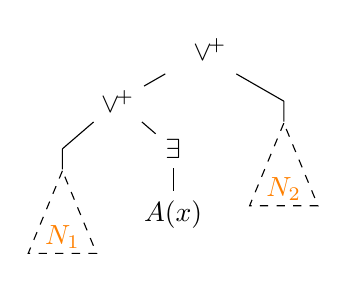
\begin{tikzpicture}[sibling distance=6em,level distance=4ex, level 2/.style={sibling distance =4em}]
			\node (pos1) {\phantom{$\vee$}$\veep$\strut}
			child { node {$\veep$}%{\rlap{$\veep$}\phantom{$\vee$}} %
				child {
					child[level distance=1ex] {node[itria] {\smash{\negf{$N_1$}}}}}
				child { node {$\exists$}
					child[level distance=5.5ex] {node {${A(x)}$}}}}
			child {
				child[level distance=1ex] {node[itria] {\smash{\negf{$N_2$}}}}};
			\end{tikzpicture}}}
}
\only<7>{
	$\bm\rightarrow$
}
\only<7>{
		\parbox[c]{2.5cm}{
		\scalebox{.65}{
			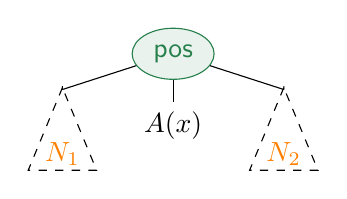
\begin{tikzpicture}[sibling distance=4em,level distance=3ex]
			\node[ellipse,draw = DarkGreen,fill = DarkGreen!10] (pos2) {\posf{$\mathsf{pos}$}}
			child {
				child [level distance=-1ex]{node[itria] {\smash{\negf{$N_1$}}}}}
			child [level distance=6ex]{node {${A(x)}$}}
			child {
				child [level distance=-1ex]{node[itria] {\smash{\negf{$N_2$}}}}};
			\end{tikzpicture}}}
}


\only<8-9>{
	{\small $(\forall x\posf{P_1}\wedgen\posf{P_2})\wedgen(\forall y{B(y)}\wedgen \posf{P_3})$}
	\parbox[c]{2.5cm}{
		\scalebox{.65}{
			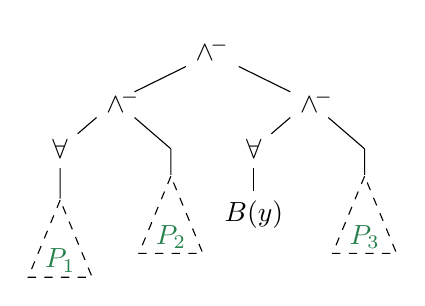
\begin{tikzpicture}[sibling distance=7em,level distance=4ex, level 2/.style={sibling distance =4em}]
			\node (neg 1) {$\wedgen$\strut}
			child { node {\rlap{$\wedgen$}\phantom{$\vee$}}
				child { node {$\forall$}
					child[level distance=3ex] {node[itria] {\smash{\posf{$P_1$}}}}}
				child {
					child[level distance=1ex] {node[itria] {\smash{\posf{$P_2$}}}}}}
			child { node {\rlap{$\wedgen$}\phantom{$\vee$}}
				child { node {$\forall$}
					child[level distance=5.5ex] {node {${B(y)}$}}}
				child {
					child[level distance=1ex] {node[itria] {\smash{\posf{$P_3$}}}}}};
			\end{tikzpicture}}}
}
\only<9>{
	$\bm\rightarrow$
}
\only<9>{
		\parbox[c]{2.5cm}{
		\scalebox{.65}{
			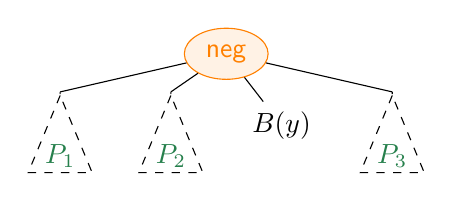
\begin{tikzpicture}[sibling distance=4em,level distance=3.2ex]
			\node[ellipse,draw = orange,fill = orange!10] (neg2) {\negf{$\mathsf{neg}$}}
			child {
				child [level distance=-1ex]{node[itria] {\smash{\posf{$P_1$}}}}}
			child {
				child [level distance=-1ex]{node[itria] {\smash{\posf{$P_2$}}}}}
			child [level distance=6ex]{node {{$B(y)$}}}
			child {
				child [level distance=-1ex]{node[itria] {\smash{\posf{$P_3$}}}}};
			\end{tikzpicture}}}
}
\end{overlayarea}
\end{frame}

\begin{frame}\frametitle{Bipolar formulas}
	
	The hierarchy can be specified for \emphdr{intuitionistic or classical} formulas. 
	
	\begin{block}{}
		Any formula in the class $\negclass{2}{C}$ / $\negclass{2}{I}$ is a classical/ intuitionistic \emph{bipolar formula}.
	\end{block}

	\bigskip\pause

	\textbf{Aside: How to polarize a formula?}
	\begin{itemize}
		\item atomic formulas are labeled either \posf{positive} or \negf{negative}
		
		\item replace all occurrences of constants and connectives with a polarized variant.
%		(If there are $n$ occurrences, there are $2^n$ ways to do this replacement.)
		\begin{itemize}
		\item in \emphdb{intuitionistic logic}: always rename false and disjunction as $\falsep$ and $\veep$ !
		\end{itemize}
	\end{itemize}
	
	\bigskip\pause

	\textbf{Example.} $(P_1 \impl P_2) \vee (Q_1 \impl
	Q_2)$ 
	\begin{itemize}
	\item $(P_1 \impl
	P_2) \veen (Q_1 \impl Q_2)$ $\leadsto$ classical bipolar.
	\item \emphdo{No polarization} yields an intuitionistic
	bipolar formula.
	\end{itemize}
\end{frame}

\section{Focusing and bipoles}

%\subsection{Focused rules}

\begin{frame}\frametitle{What is focusing?} 
	Consider again the sequent 
	\[
	\Gamma, A_1 \supset A_2\impl A_3 \supset A_4\supset A_0 \vdash B
	\]
	with $A_i$ atomic, $B$ a formula and $\Gamma$ a multiset of formulas.
	\pause\smallskip
	\begin{center}
		\emphdb{How to prove it?}
	\end{center} 
	\pause
	\begin{center}
		\emphdr{Many ways to proceed!}
	\end{center}
	\pause
	\bigskip
	\textbf{Focused rule application~\cite{andreoli92jlc}:}  
	
	\emph{commit} to repeat the $\limpl$ rule on the right premise until the
	atomic formula $A_0$ results:
	\[
	\infer[\limpl]{\Gamma, \emph{A_1 \supset A_2\impl A_3 \supset A_4\supset A_0} \vdash B}{
		\deduce{\Gamma \vdash {A_1}}{} &
		\infer[\limpl]{\Gamma, \emph{A_2\impl A_3 \supset A_4\supset A_0} \vdash B}{
			\deduce{\Gamma \vdash {A_2}}{} &
			\infer[\limpl]{\Gamma, \emph{A_3 \supset\cdots\supset A_n\supset A_0} \vdash B}{
				\deduce{\Gamma \vdash {A_3}}{} &
				\infer[\limpl]{\Gamma, \emph{A_4\supset A_0} \vdash B}{
					\Gamma \vdash {A_4} & \Gamma,\emph{A_0} \vdash B}}}}
	\]
	
\end{frame}

\begin{frame}
	\frametitle{An organisational tool}
	
	\textbf{Focusing} provides a way to restrict the proof search space while remaining \emph{complete}.
	
	\pause
	
	\begin{itemize}
		\item Identify and \emphdr{always apply} invertible introduction rules;
		
		\item \emphdr{Chain together} the other rules (non-invertible/consuming external information).
	\end{itemize}
	
	\pause
	\begin{center}
		\emphdb{$\Rightarrow$} Maximal chaining of the decomposition.
	\end{center}
	
	\pause 
	\medskip
	
	\begin{center}
		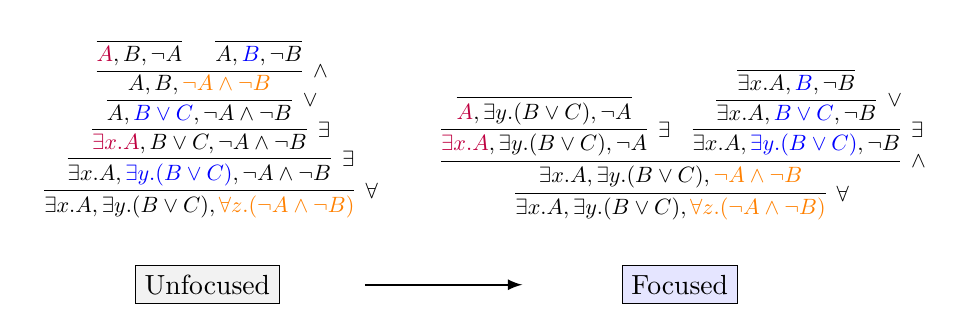
\begin{tikzpicture}
		\node (unf) at (-3,0) {
			\scalebox{.8}{
			$
			\infer[\forall]{\exists x. A, \exists y.(B \vee C), \orange{\forall z.(\neg A \wedge  \neg B)}}{
				%
				\infer[\exists]{\exists x. A, \blue{\exists y.(B \vee C)}, \neg A \wedge  \neg B}{
					%
					\infer[\exists]{\purple{\exists x. A}, B \vee C, \neg A \wedge \neg B}{
						%
						\infer[\vee]{A, \blue{B \vee C}, \neg A \wedge \neg B}{
							%
							\infer[\wedge]{A, B, \orange{\neg A \wedge  \neg B}}{
								%
								\infer[]{\purple{A}, B, \neg A}{
									%
								} &
								%
								\infer[]{A, \blue{B}, \neg B}{
									%
			}}}}}}
			$}
		};
		\node[rectangle,draw,fill = gray!10] at (-3,-2) {Unfocused};
		\uncover<5->{
			\node (foc) at (3,-0.2) {
				\scalebox{.8}{
				$
					\infer[\forall]{\exists x. A, \exists y.(B \vee C), \orange{\forall z.(\neg A \wedge  \neg B)}}{
						%
						\infer[\wedge]{\exists x. A, {\exists y.(B \vee C)}, \orange{\neg A \wedge \neg B}}{
							%
							\infer[\exists]{\purple{\exists x. A}, {\exists y.(B \vee C)}, {\neg A}}{
								%
								\infer[]{\purple{A},{\exists y.(B \vee C)}, {\neg A}}{
									%
									%
									%
						}}&
							\infer[\exists]{\exists x. A, \blue{\exists y.(B \vee C)}, {\neg B}}{
								%
								\infer[\vee]{\exists x. A, {\blue{B \vee C}, \neg B}}{
									%
									\infer[]{\exists x. A, {\blue{B}, \neg B}}{
										%
										%
										%
				}}}}}
				$}
			};
			\draw[->,>=latex,thick] (-1,-2)--(1,-2);
			\node[rectangle,draw,fill = blue!10] at (3,-2) {Focused};
		}
		\end{tikzpicture}
	\end{center}
	
\end{frame}

%%%%%%%%%%%%%%%%%%%%%%%%%%%%%%%%%%%%%%%%%%%%%%%%%%%%%
%%%%%%%%%%%%%%%%%%%%%%%%%%%%%%%%%%%%%%%%%%%%%%%%%%%%%
%%%%%%%%%%%%%%%%%%%%%%%%%%%%%%%%%%%%%%%%%%%%%%%%%%%%%
%%%%%%%%%%%%%%%%%%%%%%%%%%%%%%%%%%%%%%%%%%%%%%%%%%%%%


\begin{frame}\frametitle{\LKF~and \LJF~\cite{liang07csl,LiaMil09}}
	\textbf{Two kinds of focused sequents}
		
	\begin{itemize}
		\item 
		\emphdr{$\Downarrow$ sequents} to decompose the formula \emph{under focus}
		\begin{center}
	
		$\jLf{\Gamma}{B}{\Delta}$ with a left focus on $B$
		
		$\jRf{\Gamma}{B}{\Delta}$ with a right focus on $B$
		
		\end{center}
		\smallskip
		
		When the conclusion of an introduction rule, then that
		rule introduced $B$.
		
		\medskip
		
			\item \emphdr{$\Uparrow$ sequents}  for invertible introduction rules
			\begin{center}
				$\jUnf{\Gamma_1}{\Gamma_2}{\Delta_1}{\Delta_2}$
			\end{center}
		
		\smallskip
		
%		The particular sequent 
%		$\jUnf{\Gamma}{\cdot}{\cdot}{\Delta}$
%		is called a \emph{border} sequent.
			\end{itemize}
		
		\bigskip\pause
		
		\textbf{Example of rules:}
		
		\begin{center}
		\begin{tabular}{c@{\qquad\qquad}c}
			$\infer{\jLf{\Gamma}{B_1 \supset B_2}{\Delta}}{\jRf{\Gamma}{B_1}{\Delta}& \jLf{\Gamma}{B_2}{\Delta}} $
			&
			$\infer{\jUnf{\Gamma_1}{\Gamma_2}{B_1 \supset B_2}{\Delta}}{\jUnf{\Gamma_1}{\Gamma_2,B_1}{B_2}{\Delta}}$
			\\
			\emph{non-invertible} 
			&
			\emphdr{invertible} 
		\end{tabular}
		\end{center}

\end{frame}

\begin{frame}\frametitle{\LKF~and \LJF~\cite{liang07csl,LiaMil09}}
	\textbf{The dynamic of proof search:}
	\begin{itemize}
		\item<1-> A formula is put \empha{under focus}
		\begin{itemize}
		\item[]
		$
		\labelleft{Decide:}\qquad
		\infer[\kern -2pt D_l]{\jUnf{\Gamma,N}{\cdot}{\cdot}{\Delta}}{\jLf{\Gamma,N}{N}{\Delta}}
		\qquad
		\infer[\kern -2 pt D_r]{\jUnf{\Gamma}{\cdot}{\cdot}{P,\Delta}}{\jRf{\Gamma}{P}{\Delta}}
		$
		\end{itemize}
		
		\item<2-> Focus is transferred from conclusion to premises until 
		\begin{itemize}
			\item<3-> either the \emphdr{focused phase ends}
			
			\smallskip
			$
			\labelleft{Release:}\qquad
			\infer[R_l]{\jLf{\Gamma}{P}{\Delta}}{\jUnf{\Gamma}{P}{\cdot}{\Delta}}
			\qquad
			\infer[R_r]{\jRf{\Gamma}{N}{\Delta}}{ \jUnf{\Gamma}{\cdot}{N}{\Delta}}
			$
			
			\item<4->  or the \emphdr{derivation ends}
			
			\smallskip
			$
			\labelleft{Initial:}\qquad
			\infer[I_l]{\jLf{\Gamma}{N}{N,\Delta}}{N \; \mbox{atomic}}
			\qquad
			\infer[I_r]{\jRf{\Gamma,P}{P}{\Delta}}{P \; \mbox{atomic}}
			$
		\end{itemize}
	
		\item<5-> Once the focus is released, the formula is \emphb{eagerly decomposed} into subformulas, 
		\pause[6]
		which are ultimately \emphdb{stored} in the context.
		\begin{itemize}
			\item[]
			$
			\labelleft{Store:}\qquad
			\infer[S_l]{\jUnfamb{\Gamma_1}{\Gamma_2,P}{\null}}{\jUnfamb{\Gamma_1,P}{\Gamma_2}{\null}}
			\qquad
			\infer[S_r]{\jUnf{\Gamma}{\cdot}{N,\Delta_1}{\Delta_2}}{\jUnf{\Gamma}{\cdot}{\Delta_1}{N,\Delta_2}}
			$
		\end{itemize}

		\medskip
		\item<7->[$\Rightarrow$] Sequent derivations are organized into \emphdr{synchronous/asynchronous phases}
		\item<8->[$\Rightarrow$] \emphdr{Synthetic rules} result from looking only at {border sequents}: $\jUnf{\Gamma}{\cdot}{\cdot}{\Delta}$~\cite{DBLP:conf/lpar/Chaudhuri08}
		\end{itemize}
\end{frame}

%\begin{frame}
%	\frametitle{\LJF: Identity rules and Structural rules}
%	\[
%	\labelleft{Initial:}\qquad
%	\infer[I_l]{\jLf{\Gamma}{N}{N}}{N \; \mbox{atomic}}
%	\qquad
%	\infer[I_r]{\jRf{\Gamma,P}{P}}{P \; \mbox{atomic}}
%	\]
%	\[
%	\labelleft{Cut:}\qquad
%	\infer[Cut]{\jUnf{\Gamma}{\cdot}{\cdot}{E}}
%	{\jUnf{\Gamma}{\cdot}{B}{\cdot}\qquad \jUnf{\Gamma}{B}{\cdot}{E}}
%	\]
%	\[
%	\labelleft{Decide:}\qquad
%	\infer[\kern -2pt D_l]{\jUnf{\Gamma,N}{\cdot}{\cdot}{E}}{\jLf{\Gamma,N}{N}{E}}
%	\qquad
%	\infer[\kern -2 pt D_r]{\jUnf{\Gamma}{\cdot}{\cdot}{P}}{\jRf{\Gamma}{P}}
%	\]
%	\[
%	\labelleft{Release:}\qquad
%	\infer[R_l]{\jLf{\Gamma}{P}{E}}{\jUnf{\Gamma}{P}{\cdot}{E}}
%	\qquad
%	\infer[R_r]{\jRf{\Gamma}{N}}{ \jUnf{\Gamma}{\cdot}{N}{\cdot}}
%	\]
%	\[
%	\labelleft{Store:}\qquad
%	\infer[S_l]{\jUnfamb{\Gamma}{\Theta,C}{\null}}{\jUnfamb{\Gamma,C}{\Theta}{\null}}
%	\qquad
%	\infer[S_r]{\jUnf{\Gamma}{\cdot}{E}{\cdot}}{\jUnf{\Gamma}{\cdot}{\cdot}{E}}
%	\]
%	Here,
%	$P$ is a positive formula;
%	$N$ is a negative formula;
%	$C$ is either a negative formula or a positive atom;
%	$E$ is either a positive formula or a negative atom; and
%	$B$ is an unrestricted polarized formula.
%\end{frame}
%
%\begin{frame}
%	\frametitle{\LJF: Asynchronous Introduction Rules}
%	%  \vspace*{-20pt}
%	\[
%	\infer{\jUnfG{\cdot}{B_1 \supset B_2}}{\jUnfG{B_1}{B_2}} %[\supset_r]
%	\qquad
%	\infer{\jUnfG{\cdot}{B_1 \wedgen B_2}} %[\wedgen_r]
%	{\jUnfG{\cdot}{B_1} \quad \jUnfG{\cdot}{B_2}}
%	\qquad
%	\infer{\jUnfG{\cdot}{\truen}}{} %[\truen_r]
%	\]
%	\hfill
%	\[
%	\infer{\jUnfGamb{\Theta,\falsep}}{} %[\falsep_l]
%	\qquad
%	\infer{\jUnfGamb{\Theta,B_1\veep B_2}} %[\veep_l]
%	{\jUnfGamb{\Theta,B_1}\quad \jUnfGamb{\Theta,B_2}}
%	\]
%	\hfill
%	\[
%	\infer{\jUnfGamb{\Theta,B_1\wedgep B_2}}{\jUnfGamb{\Theta,B_1,B_2}} %[\wedgep_l]
%	\qquad
%	\infer{\jUnfGamb{\Theta,\truep}}{\jUnfGamb{\Theta}} %[\truep_l]
%	\]
%	\hfill
%	\[
%	\infer[$\dag$]{\jUnfG{\cdot}{\forall x.B}}{\jUnfG{\cdot}{[y/x]B}} %[\forall_r]
%	\qquad
%	\infer[$\dag$]{\jUnfGamb{\Theta,\exists x.B}}{\jUnfGamb{\Theta,[y/x]B}} %[\exists_l]
%	\]
%	
%	\hfill
%	
%	Here, 
%	$\Gamma$ and $\Delta_2$ ranges over multisets of polarized formulas,\\
%	\qquad\ $\Theta$ and $\Delta_1$ ranges over \emph{lists} of polarized formulas
%	%\qquad\ $\Rscr$ is a right hand side with exactly one formula.
%	
%	%\hfill
%	
%	
%	$\dag$ The usual eigenvariable restriction applies to $y$.
%	
%	\hfill
%	
%\end{frame}
%
%\begin{frame}
%	\frametitle{\LJF: Synchronous Introduction Rules}
%	\[
%	\infer{\jLfG{\forall x.B}}{\jLfG{[t/x]B}} %[\forall_l]
%	\qquad
%	\infer{\jRfG{\exists x.B}}{\jRfG{[t/x]B}} %[\exists_r]
%	\]
%	
%	\[
%	\infer{\jRfG{B_1 \veep B_2}}{\jRfG{B_i}} %[\veep_r]
%	\qquad
%	\infer[i \in \{1,2\}]{\jLfG {B_1 \wedge^- B_2}}{\jLfG{B_i}} %[\wedgen_l]
%	\]
%	
%	\[ 
%	\infer{\jLfG{B_1 \supset B_2}}{\jRfG{B_1}\quad \jLfG{B_2}} %[\supset_l]$\ddag$
%	\]
%	
%	\[
%	\infer[$\ddag$]{\jRfG{\truep}}{} %[\truep_r]
%	\qquad
%	\infer{\jRfG{B_1 \wedge^+ B_2}}{\jRfG{B_1}\quad\jRfG{B_2}} %[\wedgep_r]%$\ddag$
%	\]
%	
%	Here, $E$ denotes either a positive formula or a negative atom.
%	
%	%$\ddag$ We will see later why these rules are classified as ``possibly
%	%non-invertible''. 
%	
%\end{frame}
%


%%%%%%%%%%%%%%%%%%%%%%%%%%%%%%%%%%%%%%%%%%%%%%%%%%%%%%%%%%%%%%%%%
%%%%%%%%%%%%%%%%%%%%%%%%%%%%%%%%%%%%%%%%%%%%%%%%%%%%%%%%%%%%%%%%%
%%%%%%%%%%%%%%%%%%%%%%%%%%%%%%%%%%%%%%%%%%%%%%%%%%%%%%%%%%%%%%%%%
%\subsection{Synthetic rules}
%
%\begin{frame}
%	\frametitle{Synthetic rules}
%	
%	\emph{Synthetic inference rule}~\cite{DBLP:conf/lpar/Chaudhuri08}, where the focused formula is rewritten into (some of) its subformulas.
%	
% That is, a
%	synthetic rule is built from a collect of focused 
%	rules in which the conclusion and the premises are border sequents.
%	\[
%	\infer[decide]{\jUnf{\Gamma}{\cdot}{\cdot}{\Delta}}{
%		\deduce{\qquad\ldots \qquad \Downarrow \qquad\ldots \qquad}{
%			\deduce{\qquad\ldots \qquad \vdots \strut\qquad\ldots \qquad}{
%				\deduce{\qquad\ldots \qquad \Uparrow \qquad\ldots \qquad}{
%					\ldots\qquad\jUnf{\Gamma_i}{\cdot}{\cdot}{\Delta_i}\qquad\ldots}
%	}}}
%	\]
%	The corresponding synthetic rule is of the form
%	\[
%	\infer{\Seq{\Gamma}{\Delta}}{\ldots\qquad\Seq{\Gamma_i}{\Delta_i}\qquad\ldots}
%	\]
%	Of course, the polarized formulas here need to be replaced by their
%	corresponding unpolarized form.
%\end{frame}



%%%%%%%%%%%%%%%%%%%%%%%%%%%%%%%%%%%%%%%%%%%%%%%%%%%%%%%%%%%%%%%%%
%%%%%%%%%%%%%%%%%%%%%%%%%%%%%%%%%%%%%%%%%%%%%%%%%%%%%%%%%%%%%%%%%
%%%%%%%%%%%%%%%%%%%%%%%%%%%%%%%%%%%%%%%%%%%%%%%%%%%%%
%%%%%%%%%%%%%%%%%%%%%%%%%%%%%%%%%%%%%%%%%%%%%%%%%%%%%

\begin{frame}\frametitle{Bipole}
	Let $B$ be a polarized negative (classical or intuitionistic) formula.
	
	\begin{block}{}
		A \emph{bipole for $B$} is a synthetic inference rule  
		corresponding to a derivation (in $\LKF$ or $\LJF$)
		\begin{enumerate}
			\item<2-> starting with a decide on $B$;
			\item<3-> in which no synchronous rule occurs above an asynchronous rule;
			\item<4-> and only atomic formulas are stored.
		\end{enumerate}
	\end{block} 

	\begin{overlayarea}{\textwidth}{5cm}
		\begin{tikzpicture}
		\uncover<5->{
		\node at (-1.9,2.5) {$\jUnf{\Gamma_1}{\cdot}{\cdot}{\Delta_1}  \quad\ldots\quad \jUnf{\Gamma_n}{\cdot}{\cdot}{\Delta_n}$};
		\node at (-1.5,-1.4) {$\infer[\kern -2pt D_l]{
				\jUnf{\Gamma,B}{\cdot}{\cdot}{\Delta}}{
				\jLf{\Gamma,B}{B}{\Delta}}$};
		}
		%
		\only<5>{
		\node at (0,0) {\includegraphics[scale=0.65]{focusing}};
		}
		%
		\only<6>{
		\node at (-2.2,0.7) {\includegraphics[scale=0.65]{focusing2}};
		%
		\node at (4,1) {\textbf{Corresponding synthetic rule}};
		\node at (4,0.5) {(in $\LK$ or $\LJ$)};
		\node at (4,-0.5) {
			$\infer{\Gamma \seq \Delta}{\Gamma_1 \seq \Delta_1 \quad\ldots\quad \Gamma_n\seq\Delta_n}$};
		}
		\end{tikzpicture}
	\end{overlayarea}
\end{frame}



%%%%%%%%%%%%%%%%%%%%%%%%%%%%%%%%%%%%%%%%%%%%%%%%%%%%%
%%%%%%%%%%%%%%%%%%%%%%%%%%%%%%%%%%%%%%%%%%%%%%%%%%%%%
%%%%%%%%%%%%%%%%%%%%%%%%%%%%%%%%%%%%%%%%%%%%%%%%%%%%%
%%%%%%%%%%%%%%%%%%%%%%%%%%%%%%%%%%%%%%%%%%%%%%%%%%%%%

\section{Axioms-as-rules revisited}

\begin{frame}\frametitle{1st result: Bipolar $\longleftrightarrow$ Bipole}
	
	Let $B$ be a polarized negative (classical or intuitionistic) formula.
	
	\begin{block}{}
		\textbf{Theorem:} 
		\begin{itemize}
			\item If $B$ is bipolar, then \emphdr{any} synthetic inference rule for $B$ is a \emph{bipole}.
			
			\item If \emphdr{every} synthetic inference rule for $B$ is a bipole
			then $B$ is \emph{bipolar}.
		\end{itemize}
	\end{block}

	\bigskip
	
	\textbf{Prototype implementation:}

	\lP~\cite{miller12proghol,nadathur88iclp} executable specification of a
	predicate that relates a bipolar formula to its various bipoles.
	\begin{itemize}
		\item[$\Rightarrow$] compact given the nature of \lP
		\item[$\Rightarrow$]
		explicit about the scope of bindings for schematic variables and
		eigenvariables.
	\end{itemize}

	
\end{frame}

\begin{frame}
	\frametitle{2nd result: Cut admissibility}
	Let $\axioms$ be a set of bipolar formulas.
	\smallskip
	
	\emphdr{$\LK\tup{\axioms}$/$\LJ\tup{\axioms}$} denotes the
	extension of $\LK$/$\LJ$ with the synthetic inference rules 
	corresponding to a bipole for each $B\in\axioms$.
	
	\begin{block}{}
		\textbf{Theorem:}
		The cut rule is admissible for the proof systems
		$\LK\tup{\axioms}$/$\LJ\tup{\axioms}$.
	\end{block}

	\emphdo{Note:} the proof is \emph{simple}!
	\smallskip
	
	It is a direct consequence of (polarized) cut admissibility in $\LKF$/$\LJF$.
		\[
%		\labelleft{Cut:}\qquad
		\infer[Cut]{\jUnf{\Gamma}{\cdot}{\cdot}{\Delta}}
		{\jUnf{\Gamma}{\cdot}{B}{\Delta}\qquad \jUnf{\Gamma}{B}{\cdot}{\Delta}}
		\]
\end{frame}



%\begin{frame}{TODO}
%	\begin{definition}[Rules from polarized axioms]
%		Let $\tup{\delta,\axioms}$ be a finite set of bipolar formulas.
%		%
%		We define $\LK\tup{\delta,\axioms}$ to be the extension of \LK with
%		inference rules derived from the polarized theory
%		$\tup{\delta,\axioms}$ as follows.
%		%
%		For every $B\in\axioms$ and every synthetic inference rule for $B$,
%		say, 
%		\[
%		\infer[,]{\jUnf{\Gamma}{}{}{\Delta}}
%		{\jUnf{\Gamma_1}{}{}{\Delta_1} & \ldots & 
%			\jUnf{\Gamma_n}{}{}{\Delta_n}}
%		\]
%		we place in $\LK\tup{\delta,\axioms}$ the inference
%		rule
%		\[
%		\infer[.]{\Gamma\vdash\Delta}
%		{\Gamma_1\vdash \Delta_1 & \ldots & 
%			\Gamma_n\vdash \Delta_n}
%		\]
%		%
%		Since $\Gamma, \Gamma_1,\ldots, \Gamma_n, \Delta, \Delta_1, \ldots,
%		\Delta_n$ are composed of either atomic formulas or schematic
%		(context) variables, there are no logical connectives that need to be
%		``de-polarize'' when moving from the first inference rule above to the
%		second.
%	\end{definition}
%	
%	
%\end{frame}
%%%%%%%%%%%%%%%%%%%%%%%%%%%%%%%%%%%%%%%%%%%%%%%%%%%%%
%%%%%%%%%%%%%%%%%%%%%%%%%%%%%%%%%%%%%%%%%%%%%%%%%%%%%
%%%%%%%%%%%%%%%%%%%%%%%%%%%%%%%%%%%%%%%%%%%%%%%%%%%%%
%%%%%%%%%%%%%%%%%%%%%%%%%%%%%%%%%%%%%%%%%%%%%%%%%%%%%

\begin{frame}\frametitle{Rules from axioms}
	
	\scalebox{.8}{
		\begin{tikzpicture}
		\tikzstyle{operation}=[->,>=latex,thick]
		\tikzstyle{state}=[rectangle,draw,thick, rounded corners=5pt, text width = 1.6cm, align=center]
		\tikzstyle{etiquette}=[rectangle,draw,thick,dotted]
		%%rectangles
		%\draw [fill=red!20, thick] (5,-0.5) rectangle (8,-3.5);
		%\draw [fill=blue!20, thick, rounded corners=7pt] (-1.5,-0.5) rectangle (1.5,0.5);
		%%points
		\uncover<2->{
			\node[state, fill=gray!20] (i) at (0,0)  {Unpolarized\\Axiom};
		}
		\only<2,19>{
			\node[right = of i] {$\forall x (((P_1(x) \impl P_2(x)) \wedge Q(x)) \impl\exists y R(x,y))$};
		}
		%
		\uncover<4->{
			\node[state, fill=blue!20] (ii) at (2.5,2) {Polarized\\Axiom};
			\node[state, fill=blue!20] (ii') at (2.5,-2) {Polarized\\Axiom};
			%	\draw[dotted,thick] (2.5,1.2)--(2.5,-1.2);
		}
		%
		\uncover<3->{
			\draw[operation] (i)--(ii) node[etiquette] at (0.7,1.2) {Polarizing};
			\draw[operation] (i)--(ii');
		}
		\only<3-6,11-12,16-17>{
			\draw[operation,dotted] (i)--(2,0.8);
			\draw[operation,dotted] (i)--(2,0);
			\draw[operation,dotted] (i)--(2,-0.8);
		}
		%
		\only<4-6,11,16>{
			\node[right] at (2,0.8) {$\negf{\bm\forall}x (((\posf{P_1}(x) \negf{\bm\impl} \negf{P_2}(x)) \posf{\bm\wedgep} \posf{Q}(x)) \negf{\bm\impl}\posf{\bm\exists}y \posf{R}(x,y))$};
		}
		\only<4-5,11-12,16>{
			\node[right] at (2,0) {$\negf{\bm\forall}x (((\posf{P_1}(x) \negf{\bm\impl} \negf{P_2}(x)) \negf{\bm\wedgen} \negf{Q}(x)) \negf{\bm\impl}\posf{\bm\exists}y \posf{R}(x,y))$};
		}
		\only<4-5,11,16-17>{
			\node[right] at (2,-0.8) {$\negf{\bm\forall}x (((\posf{P_1}(x) \negf{\bm\impl} \negf{P_2}(x)) \negf{\bm\wedgen} \posf{Q}(x)) \negf{\bm\impl}\posf{\bm\exists}y \posf{R}(x,y))$};
		}
		%
		\uncover<5->{
			\node[etiquette] at (4.5,3) {Is it bipolar?};
		}
		%
		\uncover<6-10,12-15,19->{
			\draw[thick] (ii)--(4.5,2) node[circle,draw,fill=green!40] {$\bm\checkmark$};
		}
		\uncover<17-20>{
			\draw[thick] (ii')--(4.5,-2) node[circle,draw,fill=red!40] {$\bm\times$};%node[etiquette] 
		}
		%
		\uncover<7-10,13-15,19->{
			\node[state, fill=green!20] (iii) at (6.5,2) {Bipole\\in \LKF}; 
			\draw[operation] (4.85,2)--(iii);
		}
		\only<7-9>{
			\node[] at (8.5,-0.5) {$
				\infer[\forall_l]{\jLf{\Gamma}{\negf{\bm\forall}x (((\posf{P_1}(x) \negf{\bm\impl} \negf{P_2}(x)) \posf{\bm\wedgep} \posf{Q}(x)) \negf{\bm\impl}\posf{\bm\exists}y \posf{R}(x,y))}{}{\Delta}}{
					\infer[\impl_l]{{\jLf{\Gamma}{((P_1(t) \impl P_2(t)) \wedgep Q(t)) \impl \exists y R(t,y)}{}{\Delta}}}{
						\infer[\wedgep_r]{\jRf{\Gamma}{(P_1(t) \impl P_2(t)) \wedgep Q(t)}{\Delta}}{
							\infer[\krelease_r]{{\jRf{\Gamma}{P_1(t)\impl P_2(t)}{\Delta}}}{
								\infer[\impl_r]{\jUnf{\Gamma}{\cdot}{P_1(t)\impl P_2(t)}{\Delta}}{
									\infer[\kstore_l]{\jUnf{\Gamma}{P_1(t)}{P_2(t)}{\Delta}}{
										\infer[\kstore_r]{\jUnf{\Gamma,P_1(t)}{\cdot}{P_2(t)}{\Delta}}{
											\deduce{\jUnf{\Gamma,\posf{P_1(t)}}{\cdot}{\cdot}{\negf{P_2(t)},\Delta}}{}
										}
									}
								}
							} 
							& 
							\infer[\kinit_r]{\jRf{\Gamma}{\posf{Q(t)}}{\Delta}}{}
						} 
						& 
						\infer[\krelease_l]{\jLf{\Gamma}{\exists y R(t,y)}{\Delta}}{
							\infer[\exists_l]{\jUnf{\Gamma}{\exists y R(t,y)}{\cdot}{\Delta}}{
								\infer[\kstore_l]{\jUnf{\Gamma}{R(t,z)}{\cdot}{\Delta}}{
									\deduce{\jUnf{\Gamma, \posf{R(t,z)}}{\cdot}{\cdot}{\Delta}}{}
								}
							}
						}
					}
				}
				$};
		}
		%
		\only<13-14>{
			\node[] at (8.5,-0.5) {$
				\infer[\forall_l]{\jLf{\Gamma}{\negf{\bm\forall}x (((\posf{P_1}(x) \negf{\bm\impl} \negf{P_2}(x)) \negf{\bm\wedgen} \negf{Q}(x)) \negf{\bm\impl}\posf{\bm\exists}y \posf{R}(x,y))}{}{\Delta}}{
					\infer[\impl_l]{{\jLf{\Gamma}{((P_1(t) \impl P_2(t)) \wedgen Q(t)) \impl \exists y R(t,y)}{}{\Delta}}}{
						\infer[\krelease_r]{\jRf{\Gamma}{(P_1(t) \impl P_2(t)) \wedgen Q(t)}{\Delta}}{
							\infer[\wedgen_r]{\jUnf{\Gamma}{\cdot}{(P_1(t) \impl P_2(t)) \wedgen Q(t)}{\Delta}}{
								\infer[\impl_r]{\jUnf{\Gamma}{\cdot}{P_1(t)\impl P_2(t)}{\Delta}}{
									\infer[\kstore_l]{\jUnf{\Gamma}{P_1(t)}{P_2(t)}{\Delta}}{
										\infer[\kstore_r]{\jUnf{\Gamma,P_1(t)}{\cdot}{P_2(t)}{\Delta}}{
											\deduce{\jUnf{\Gamma,\posf{P_1(t)}}{\cdot}{\cdot}{\negf{P_2(t)},\Delta}}{}
										}
									}
								}
								& 
								\infer[\kstore_r]{\jUnf{\Gamma}{\cdot}{Q(t)}{\Delta}}{
									\deduce{\jUnf{\Gamma}{\cdot}{\cdot}{\negf{Q(t)}, \Delta}}{}
								}
							} 
						} 
						& 
						\infer[\krelease_l]{\jLf{\Gamma}{\exists y R(t,y)}{\Delta}}{
							\infer[\exists_l]{\jUnf{\Gamma}{\exists y R(t,y)}{\cdot}{\Delta}}{
								\infer[\kstore_l]{\jUnf{\Gamma}{R(t,z)}{\cdot}{\Delta}}{
									\deduce{\jUnf{\Gamma, \posf{R(t,z)}}{\cdot}{\cdot}{\Delta}}{}
								}
							}
						}
					}
				}
				$};
		}
		%
		\uncover<9-10,14-15,19->{
			\node[state, fill=orange!20] (iv) at (9.5,2) {Inference\\rule for \LK};
		}
		\uncover<8-10,14-15,19->{
			\draw[operation] (iii)--(iv) node[etiquette] at (8,3) {Synthesizing};
		}
		\only<9-10>{
			\node[draw] at (11,1) {$
				\infer[]{\Gamma = \Gamma', \emphdr{Q(t)}\seq\Delta}{
					\Gamma, \emphdr{P_1(t)}\seq\emphdr{P_2(t)},\Delta
					& 
					\Gamma, \emphdr{R(t,z)}\seq\Delta}
				$};
		}
		%
		\only<14-15>{
			\node[draw] at (10.5,1) {$
				\infer[]{\Gamma\seq\Delta}{
					\Gamma, \emphdr{P_1(t)}\seq\emphdr{P_2(t)},\Delta
					&
					\Gamma \seq\emphdr{Q(t)},\Delta
					& 
					\Gamma, \emphdr{R(t,z)}\seq\Delta}
				$};
		}
		%
		\only<19>{
			\node[draw] at (11.5,0) {$
				\infer[]{\Gamma = \Gamma', \emphdr{Q(t)}\seq\Delta}{
					\Gamma, \emphdr{P_1(t)}\seq\emphdr{P_2(t)},\Delta
					& 
					\Gamma, \emphdr{R(t,z)}\seq\Delta}
				$};
			\node[draw] at (10.5,-1.5) {$
				\infer[]{\Gamma\seq\Delta}{
					\Gamma, \emphdr{P_1(t)}\seq\emphdr{P_2(t)},\Delta
					&
					\Gamma \seq\emphdr{Q(t)},\Delta
					& 
					\Gamma, \emphdr{R(t,z)}\seq\Delta}
				$};
		}
		%
		%\uncover<20>{
		%\node[text width = 1cm,align=center, fill=gray!20] at (0,-1)  {$\axioms$};
		%\node[fill=blue!20] at (2.5,1) {$\tup{\delta,\axioms}$};
		%\node[fill=orange!20] at (9.5,1) {$\LK\tup{\axioms}$};
		%}
		\end{tikzpicture}
	}
	
	
\end{frame}





\section{Examples}
\subsection{Geometric axioms}

\begin{frame}\frametitle{Geometric axioms as bipoles}
	
\only<1>{\emphdr{Geometric implication:}}
%
\only<2->{\emphdo{Polarized geometric implication:}}
		
%\begin{overlayarea}{\textwidth}{1cm}
\only<1>{
		\[\forall \overline{z} (P_1 \wedge \ldots \wedge P_m \, \impl \, \exists \overline{x}_1 M_1 \vee \ldots \vee \exists \overline{x}_n M_n ) 
		\]
}	
\only<2>{
\[\negf{\forall \overline{z}} (P_1^{\pm} \wedgepn \ldots \wedgepn P_m^{\pm} \, \negf{\impl} \, \posf{\exists \overline{x}_1} \hat{M_1} \veepn \ldots \veepn \posf{\exists \overline{x}_n} \hat{M_n} )
		\]
}
\only<3>{
	$$
	\negf{\forall \overline{z}} (\posf{P_1^{+}} \posf{\wedgep} \ldots \posf{\wedgep} \posf{P_m^{+}} \, \negf{\impl} \, \posf{\exists \overline{x}_1} \hat{M_1} \veepn \ldots \veepn \posf{\exists \overline{x}_n} \hat{M_n} ) \, ,
	$$
}
\only<4>{
	$$
	\negf{\forall \overline{z}} (\negf{P_1^{-}} \wedgepn \ldots \wedgepn \negf{P_m^{-}} \, \negf{\impl} \, \posf{\exists \overline{x}_1} \hat{M_1} \veepn \ldots \veepn \posf{\exists \overline{x}_n} \hat{M_n} ) \, ,
	$$
}
%\end{overlayarea}

\bigskip

\begin{overlayarea}{\textwidth}{4cm}
\only<1>{
\begin{itemize}
	\item $P_i$ atomic;
	\item $M_j=Q_{j_1}\wedge\ldots\wedge Q_{j_{k_{j}}}$, $Q_{j_k}$ atomic; 
	\item none of the variables in the vectors $\overline{x}_j$ are free in $P_i$.
\end{itemize}	
}
\only<2>{
\begin{itemize}
\item $\posf{P_i^+}, \negf{P_i^-}$ atomic;
\item $\hat{M_j} = Q_{j_1}^{\pm} \posf{\wedgep} \ldots \posf{\wedgep} Q_{j_{k_{j}}}^{\pm}$ , $Q_{j_k}^{\pm}$ atomic;
\item none of the variables in the vectors $\overline{x}_j$ are free in $P_i$.
\end{itemize}
}		
\only<3>{
		\emph{Corresponding bipole}:	
		$$\infer{\jUnf{\emphdr{\overline{P}},\Gamma'}{\null}{\null}{\Delta}}
		{\jUnf{\emphdr{\overline{Q}_1[\overline{y}_1/\overline{x}_1]},\Gamma}{\null} {\null}{\Delta} & \ldots & \jUnf{\emphdr{\overline{Q}_n[\overline{y}_n/\overline{x}_n]},\Gamma}{\null} {\null}  {\Delta}}
		$$
		with $\overline{P}=\{\posf{P_i^+}\}, \overline{Q_j}=\{Q_{j_k}^\pm\}$. 

		\bigskip
				
		\emphdb{Corresponding $\LK$ rule}:	
		$$\infer[GRS]{\emphdr{\overline{P}},\Gamma'\vdash \Delta}
		{\emphdr{\overline{Q}_1[\overline{y}_1/\overline{x}_1]},\Gamma\vdash\Delta & \ldots & \emphdr{\overline{Q}_n[\overline{y}_n/\overline{x}_n]},\Gamma\vdash\Delta}
		$$
	}
	
	\only<4>{
		\emph{Corresponding bipole}:	
		$$\infer[m+n\mbox{ premises}]{\jUnf{\Gamma}{\null}{\null}{\Delta}}
		{\jUnf{\emphdr{\overline{Q}_j[\overline{y}_j/\overline{x}_j]},\Gamma}{\null} {\null}{\Delta} & \ldots &\jUnf{\Gamma}{\null} {\null}{\emphdr{P_i},\Delta} }
		$$
with $\overline{Q_j}=\{Q_{j_k}\}$. 

		\bigskip
				
		\emphdb{Corresponding $\LK$ rule}:	
		$$\infer[m+n\mbox{ premises}]{\Gamma\vdash \Delta}
		{\emphdr{\overline{Q}_j[\overline{y}_j/\overline{x}_j]},\Gamma\vdash \Delta & \ldots & \Gamma\vdash \emphdr{P_i},\Delta}
		$$		
		}
\end{overlayarea}
	
\end{frame}

\begin{frame}\frametitle{Co-geometric axioms as bipoles}

\emphdo{Polarized co-geometric implication:}

	\only<1>{
		$$
		\negf{\forall \overline{z}} (\negf{\forall \overline{x}_1} \hat{M_1} \wedgepn \ldots \wedgepn \negf{\forall \overline{x}_n} \hat{M_n}  \, \negf{\impl} \, \negf{P_1^{-} \veen} \ldots \negf{\veen P_m^{-}} ) \, ,
		$$
		with $\hat{M_j}=Q_{j_1}^\pm\negf{\veen}\ldots\negf{\veen} Q_{j_{k_j}}^\pm$.
	}
	\only<2>{
		$$
		\negf{\forall \overline{z}} (\negf{\forall \overline{x}_1} \hat{M_1} \wedgepn \ldots \wedgepn \negf{\forall \overline{x}_n} \hat{M_n}  \, \negf{\impl} \, \posf{P_1^{+}} \veepn \ldots \veepn \posf{P_m^{+}} ) \, ,
		$$
		with $\hat{M_j}=Q_{j_1}^\pm\negf{\veen}\ldots\negf{\veen} Q_{j_{k_j}}^\pm$.
	}
	
		\bigskip
\begin{overlayarea}{\textwidth}{4cm}		
		\emph{Corresponding bipole}:
		\only<1>{	
		$$
		\infer
		{\jUnf{\Gamma}{\null}{\null} { \emphdr{\overline{P}}, \Delta'}}
		{\jUnf{\Gamma}{\null}{\null} { \emphdr{\overline{Q}_1[\overline{y}_1/\overline{x}_1]}, \Delta} & \ldots &  \jUnf{\Gamma}{\null}{\null}  {\emphdr{\overline{Q}_n[\overline{y}_n/\overline{x}_n]},  \Delta}}
		$$
		}
		\only<2>{
		$$
		\infer[m+n\mbox{ premises}]
		{\jUnf{\Gamma}{\null}{\null} { \Delta}}
		{\jUnf{\Gamma}{\null}{\null} { \emphdr{\overline{Q}_j[\overline{y}_j/\overline{x}_j]}, \Delta} & \ldots &  \jUnf{\Gamma, \emphdr{P_i}}{\null}{\null}  { \Delta}}
		$$
		}
		
		\bigskip
				
		\emphdb{Corresponding $\LK$ rule}:
		\only<1>{	
		$$
		\infer[co-GRS_c]
		{\Gamma\vdash \emphdr{\overline{P}}, \Delta'}
		{\Gamma\vdash \emphdr{\overline{Q}_1[\overline{y}_1/\overline{x}_1]}, \Delta & \ldots & \Gamma\vdash\emphdr{\overline{Q}_n[\overline{y}_n/\overline{x}_n]},  \Delta}
		$$
		}
	
	\only<2>{
		$$
		\infer[m+n\mbox{ premises}]
		{\Gamma\vdash \Delta}
		{\Gamma\vdash \emphdr{\overline{Q}_j[\overline{y}_j/\overline{x}_j]}, \Delta & \ldots &  \Gamma, \emphdr{P_i}\vdash \Delta}
		$$
	}
\end{overlayarea}	
\end{frame}

\subsection{Universal axioms}
\begin{frame}\frametitle{Universal axioms as bipoles}
\only<1>{\[
		\forall \overline{z}(P_1 \wedge \ldots \wedge P_m \, \impl \, Q_1\vee \ldots \vee Q_n)
		\]
}
	
\only<2>{\[
		\negf{\forall \overline{z}}(P_1^{\pm} \wedgepn \ldots \wedgepn P_m^{\pm} \, \negf{\impl} \, Q_1^{\pm} \veepn \ldots \veepn Q_n^{\pm})
		\]
}

\only<3-4>{\[
	\negf{\forall \overline{z}}(\posf{P_1^{+}} \posf{\wedgep} \ldots \posf{\wedgep} \posf{P_m^{+}} \, \negf{\impl} \, Q_1^{\pm} \posf{\veep} \ldots \posf{\veep} Q_n^{\pm})
	\]
}

\only<5-6>{\[
	\negf{\forall \overline{z}}(P_1^{\pm} \negf{\wedgen} \ldots \negf{\wedgen} P_m^{\pm} \, \negf{\impl} \, \negf{Q_1^{-} \veen} \ldots \negf{\veen Q_n^{-}})
	\]
}

\bigskip

\uncover<2->{		
More choices in the selection of polarities while still remaining bipolar formulas. 
}		

\bigskip
	
\begin{overlayarea}{\textwidth}{2cm}
\only<3-4>{	
$$	\infer[FRL_c]
	{\jUnf{\emphdr{\overline{P}}, \Gamma'} {\null}{\null} {\Delta}}
	{\jUnf{\emphdr{Q_1}, \Gamma} {\null}{\null} {\Delta} & \ldots & \jUnf{\emphdr{Q_n},  \Gamma} {\null}{\null} {\Delta}}	
	$$}
\only<4>{
\[\posf{a \in l \wedgep  a \in m  \wedgep  b \in l \wedgep  b \in m} \; \negf{\impl} \; a=b  \posf{\veep}  l = m
\]
\bigskip
\[
\infer[Uni_p]{\Gamma, \emphdr{a\in l}, \emphdr{a\in m}, \emphdr{b\in l},\emphdr{b\in m}\vdash \Delta}
{\Gamma, \emphdr{a=b}\vdash \Delta & \Gamma, \emphdr{l=m}\vdash \Delta}
\]}	
\only<5-6>{
$$\infer[FRR_c]
	{\jUnf{\Gamma}{\null}{\null}{ \emphdr{\overline{Q}},\Delta'}}
	{\jUnf{\Gamma}{\null}{\null}{ \emphdr{P_1}, \Delta} & \ldots & \jUnf{\Gamma}{\null}{\null}{ \emphdr{P_m}, \Delta}}
	$$}
\only<6>{
\[a \in l \;\negf{\wedgen}\;  a \in m\;  \negf{\wedgen} \; b \in l \; \negf{\wedgen} \; b \in m \; \negf{\impl} \; \negf{a=b  \veen  l = m}
\]
\bigskip
\[
\infer[Uni_n]{\Gamma\vdash \Delta, \emphdr{a=b}, \emphdr{l=m} }
{\Gamma\vdash \Delta,\emphdr{a\in l} & \Gamma\vdash \Delta,\emphdr{a\in m} & \Gamma\vdash \Delta,\emphdr{b\in l} & \Gamma\vdash \Delta,\emphdr{b\in m}}
\]}	
\end{overlayarea}

\end{frame}

\subsection{Horn clauses}
\begin{frame}\frametitle{Horn clauses as bipoles}
\only<1>{\[
		\forall \overline{z}(P_1 \wedge \ldots \wedge P_m \, \impl \, Q)
		\]}
	
\only<2>{\[
		\negf{\forall \overline{z}}(P_1^{\pm} \wedgepn \ldots \wedgepn P_m^{\pm} \, \negf{\impl} \, Q^{\pm})
		\]}
	
\only<3>{\[
	\negf{\forall \overline{z}}(\posf{P_1^{+}} \posf{\wedgep} \ldots \posf{\wedgep} \posf{P_m^{+}} \, \negf{\impl} \, \posf{Q^{+}} )
	\]}

\only<4>{\[
	\negf{\forall \overline{z}}(\negf{P_1^{-} \wedgen} \ldots \negf{\wedgen P_m^{-}} \, \negf{\impl} \, \negf{Q^{-}})
	\]}
		
\bigskip

\uncover<2->{		
Even more choices in the selection of polarities while still remaining bipolar formulas!}

\bigskip 

\begin{overlayarea}{\textwidth}{2cm}
\only<3>{
$$	\infer[FC]
	{\emphdr{\overline{P}}, \Gamma'\vdash\Delta}
	{\emphdr{Q}, \Gamma\vdash\Delta}	
	$$
\begin{center}
\emph{Forward-chaining} \\
\emph{\cite{Sim94,NegVPl98,DBLP:conf/tableaux/CiabattoniMS13}}
\end{center}
}

\only<4>{
$$\infer[BC]
	{\Gamma\vdash \emphdr{Q},\Delta'}
	{\Gamma\vdash \emphdr{P_1}, \Delta & \ldots &\Gamma\vdash \emphdr{P_m}, \Delta}
	$$
\begin{center}
\emph{Back-chaining}\\
\emph{\cite{Vig00}}
\end{center}}
\end{overlayarea}
\end{frame}

\subsection{Implementation}

\begin{frame}[fragile]\frametitle{Implementation -- Part I~\cite{DBLP:journals/apal/MarinMPV22}}
\textbf{Formula}

\smallskip

\only<1>{
$\forall u\forall v\forall w (\posf{\adj u v} \impl(\posf{\pth v w} \impl \posf{\pth u w}))$
\hfill\posf{Positive atoms.}
}

\only<2>{
$\forall u\forall v\forall w (\negf{\adj u v} \impl(\negf{\pth v w} \impl \negf{\pth u w}))$
\hfill\negf{Negative atoms.}
}

\medskip

\textbf{\lP\ encoding}
\begin{lstlisting}
(all u\ all v\ all w\ imp (atm (adj u v))
                     (imp (atm (path v w)) (atm (path u w)))),
\end{lstlisting}

\medskip

\textbf{Goal} 
\begin{lstlisting}
reduce (syncL Gamma F (atm B)) Premises.
\end{lstlisting}

\bigskip

\textbf{Inference rule}

\only<1>{
\[
  \infer{\emphdr{\adj X Z}, \emphdr{\pth Z Y}, L\vdash B}
        {\adj X Z, \pth Z Y, \emphdr{\pth X Y}, L\vdash B}
\]
}

\only<2>{
\[
\infer{\Gamma\vdash\emphdr{\pth X Z}}
{\Gamma\vdash\emphdr{\adj X Y} &\Gamma\vdash\emphdr{\pth Y Z}}
\]
}
\end{frame}

%\begin{frame}[fragile]\frametitle{Implementation -- Part I~\cite{DBLP:journals/apal/MarinMPV22}}
%Formula
%\[\forall u\forall v\forall w (\negf{\adj u v} \impl(\negf{\pth v w} \impl \negf{\pth u w}))\]
%\lP\ encoding
%\begin{lstlisting}
%(all u\ all v\ all w\ imp (atm (adj u v))
%                     (imp (atm (path v w)) (atm (path u w)))),
%\end{lstlisting}
%Goal 
%\begin{lstlisting}
%reduce (syncL Gamma F (atm B)) Premises.
%\end{lstlisting}
%\negf{Negative atoms.}
%
%%Substitution
%%\begin{lstlisting}
%%Premises = andp (async Gamma nil (rr (atm (adj X Y))))
%%          (andp (async Gamma nil (rr (atm (path Y Z)))) truep)
%%B        = path X Z
%%\end{lstlisting}
%
%\bigskip
%
%Inference rule
%\[
%  \infer{\Gamma\vdash\emphdr{\pth X Z}}
%        {\Gamma\vdash\emphdr{\adj X Y} &\Gamma\vdash\emphdr{\pth Y Z}}
%\]
%\end{frame}

\begin{frame}[fragile]\frametitle{Implementation -- Part II~\cite{DBLP:journals/apal/MarinMPV22}}
\textbf{Formula}

\smallskip

\only<1>{
$\forall u\forall v (\forall w(\posf{\texttt{in}~w~u}\impl \posf{\texttt{in}~w~v})\impl \posf{\texttt{subset}~u~v})$
\hfill\posf{Positive atoms.}
}

\only<2>{
	$\forall u\forall v (\forall w(\negf{\texttt{in}~w~u}\impl \negf{\texttt{in}~w~v})\impl \negf{\texttt{subset}~u~v})$
	\hfill\negf{Negative atoms.}
}

\medskip

\textbf{\lP\ encoding}
\begin{lstlisting}
(all u\ all v\ imp (all w\ imp (atm (in w u)) (atm (in w v)))
                   (atm (subset u v))).
\end{lstlisting}

\medskip

\textbf{Goal }
\begin{lstlisting}
reduce (syncL Gamma F (atm B)) Premises.
\end{lstlisting}


\bigskip

\textbf{Inference rule}

\only<1>{
\[
  \infer{\Gamma\vdash B}
           {\emphdr{\texttt{in}~w~X},\Gamma\vdash \emphdr{\texttt{in}~w~Y} &
            \emphdr{\texttt{subset}~X~Y},\Gamma\vdash B}
\]
}

\only<2>{
\[
\infer{\Gamma\vdash \emphdr{\texttt{subset}~X~Y}}
{\Gamma,~\emphdr{\texttt{in}~w~X}\vdash\emphdr{\texttt{in}~w~Y}}
\]
}


\end{frame}

%\begin{frame}[fragile]\frametitle{Implementation -- Part II~\cite{DBLP:journals/apal/MarinMPV22}}
%Formula
%\[\forall u\forall v (\forall w(\negf{\texttt{in}~w~u}\impl \negf{\texttt{in}~w~v})\impl \negf{\texttt{subset}~u~v})\]
%\lP\ encoding
%\begin{lstlisting}
%(all u\ all v\ imp (all w\ imp (atm (in w u)) (atm (in w v)))
%                   (atm (subset u v))).
%\end{lstlisting}
%Goal 
%\begin{lstlisting}
%reduce (syncL Gamma F (atm B)) Premises.
%\end{lstlisting}
%\negf{Negative atoms.}
%
%\bigskip
%
%Inference rule\[
%  \infer{\Gamma\vdash \emphdr{\texttt{subset}~X~Y}}
%        {\Gamma,~\emphdr{\texttt{in}~w~X}\vdash\emphdr{\texttt{in}~w~Y}}
%\]
%\end{frame}

\subsection{Meta-reasoning}

\frame{
\frametitle{Affine geometry}
\begin{itemize}
\item  \blue{Parallel lines}.
\xitem Affine geometry = (Euclidean geometry - congrunce) $\vee$ (projective geometry + parallels).
\xitem $l\parallel m$, $par(l,a)$.
\xitem General:
$$l\parallel l\quad l\parallel m\impl m\parallel l\quad l\parallel m\wedge m\parallel n \impl l\parallel n
$$
\xitem Incidency:
$$a\in par(l,a)\quad par(l,a)\parallel l.$$
\xitem Uniqueness
$$a \in l \wedge a \in m \wedge l \parallel m \impl l = m.$$
\xitem Substitution
$$l \parallel m \wedge m = n \impl l \parallel n.$$
\end{itemize}
}

\frame{
\frametitle{System GA}
I. General
$$\infer[Ref]{\Gamma\vdash \Delta,l\parallel l}{}\quad
\infer[Sym]{\Gamma\vdash \Delta,m\parallel l}{\Gamma\vdash \Delta,l\parallel m}\quad
\infer[Tr]{\Gamma\vdash \Delta,l\parallel n}
{\Gamma\vdash \Delta, l\parallel m\quad \Gamma\vdash \Delta,m\parallel n}$$
II. Incidency
$$\infer[IA]{\Gamma\vdash \Delta,a\in par(l,a)}{}\quad
\infer[Par]{\Gamma\vdash \Delta,par(l,a)\parallel l}{}$$
III. Uniqueness
$$\infer[Unipar]{\Gamma\vdash \Delta,l=m}
{\Gamma\vdash \Delta,a\in l\quad \Gamma\vdash \Delta,a\in m\quad \Gamma\vdash \Delta,l\parallel m}$$
IV. Substitution
$$\infer[SA]{\Gamma\vdash \Delta,l\parallel n}
{\Gamma\vdash \Delta,l\parallel m\quad \Gamma\vdash \Delta,m=n}
$$
}

\frame{
\frametitle{Meta-results~\cite{NegVPl14}}
\begin{block}{Weak version of Euclide's 5th postulate}
Given a point $a\notin l$ it does not exist a point  $b\in l$ such that $b\in par(l,a)$. \pause
$$\neg(a\in l)\impl \neg (b\in l\wedge b\in par(l,a))$$\pause
$$b\in l,b\in par(l,a)\vdash a\in l$$
\end{block} \pause
\begin{block}{GA}
The sequent $b\in l,b\in par(l,a)\vdash a\in l$  is derivable in GA.
\end{block}
{\bf Proof.} Let $\Gamma =\{b\in l,b\in par(l,a)\}$.
$$\infer[SPt]{\Gamma\vdash a\in l}
{\infer[IA]{\Gamma\vdash a\in par(l,a)}{}&
\infer[Unipar]{\Gamma\vdash l= par(l,a)}
{\infer[Initial]{\Gamma\vdash b\in l}{}&
\infer[Initial]{\Gamma\vdash b\in par(l,a)}{}&
\infer[Par]{\Gamma\vdash par (l,a)\parallel l}{}}}$$ \pause
\begin{block}{Unipar}
The sequent $b\in l,b\in par(l,a)\vdash a\in l$ is not derivable in GA-Unipar.
\end{block}
}



\section{Beyond bipoles}
\begin{frame}\frametitle{Linear systems versus hypersequents}
\begin{center}
\includegraphics[scale=0.6]{dale-elaine}
\end{center}
\end{frame}


\section{Conclusion}
\begin{frame}\frametitle{Some discussion}
	\begin{itemize}
		\item \emphdr{Dyckhoff and Negri:} \emph{every} (classical) first-order theory has a geometric conservative extension.
		\item \emphdr{In the literature:} {\em ad hoc}, propositional, structural, labeled.
		\item \emphdr{Modal} systems.
%		\item Maybe mention Barr's theorem? In fact, we can enhance Sara and von Plato's result, in the sense that if there is a polarization of an axiom turning it into an \emph{intuitionistic} bipole, then the intuitionistic and classical theorems coincide in the resulting theory.
\item \emphdr{Beyond} bipolars.
	\end{itemize}
	
\end{frame}


\begin{frame}\frametitle{To conclude}
	\begin{itemize}
		\item[$\star$] \emphdr{Synthetic inference rules} generated using \emphdb{polarization} and \emphdb{focusing} 
		provide inference rules that capture certain classes of
		\empha{axioms}.
		\item[$\star$]  In particular:
		\emphdr{bipolar formulas} correspond to inference rules for \emph{atoms}.
		\item[$\star$] As \emphdr{geometric formulas} are examples of bipolar formulas, polarized versions of such formulas yield \emphdb{well known} inference
		systems derived from geometric formulas.
		\item[$\star$]  Polarization of subsets of geometric formulas explain the \emphdr{forward-chaining} and
		\emphdr{backward-chaining} variants of their synthetic inference rules.
		\item[$\star$]  Direct proof of \emphdr{cut-elimination} for the proof systems that arise from incorporating synthetic inference rules based on polarized formulas.
		\item[$\star$]  Additionally, all of these results work equally well in both \emphdb{classical} and
		\emphdb{intuitionistic} logics using the corresponding \LKF\ and \LJF\ focused
		proof systems.
		\item[$\star$] Ecumenism?~\cite{DBLP:journals/corr/abs-2204-02076,DBLP:journals/corr/abs-2204-02199}
			\end{itemize}
\end{frame}

 \frame{
  \frametitle{Thank you!}
  
  \bigskip 
  
  \bigskip 
  
  Obrigada!!! \qquad 
  \huge
  \smiley
  
  \bigskip 
  
  \bigskip 

  
  \bigskip 
  \includegraphics[width=4cm]{Lisboa1}
  \includegraphics[width=4cm]{Lisboa2}\includegraphics[width=4cm]{Lisboa3}
  }
  
\begin{frame}[allowframebreaks]
\frametitle{References}
\bibliographystyle{alpha}
\bibliography{../biblio}
\end{frame}


\end{document}